%% Beamer slides for object detection courses
\documentclass{beamer}
\mode<presentation>{}
%%preamble
\title{Generic Object Detection}
\subtitle{From image classification to object detection}
\author{Adrien Heinzlé \newline Eca Robotics}
\usetheme{Antibes}
%% Theme a trouver pour reprendre les couleurs Eca
%\setbeamercolor*{palette secondary}{use=structure,fg=white,bg=orange}

\usepackage{biblatex}
\usepackage{graphicx,caption}
\usepackage{verbatim}

\bibliography{MIR.bib}

\begin{document}

%% title frame
\begin{frame}
    \titlepage
\end{frame}

% Current section
\AtBeginSection[ ]
{
\begin{frame}
    \tableofcontents[currentsection]
\end{frame}
}

%%% Remainder part
%\part{Remainder on Convolution Neural Networks}
%\begin{frame}
%    \partpage
%\end{frame}
%
%% normal frame
%\begin{frame}{Motivation}
%    \begin{itemize}
%        \item Object detection framework are built upon traditionnal Convolutional Neural Networks to extract features from images.
%        \item They use use Region of Interest algorithm to find objects of interest.
%        \item We will use ResNets and Xception nets.
%        \item For any remainder on convolution operations please refer to \cite[]{dumoulin_guide_2018}
%    \end{itemize}
%\end{frame}
%
%\section{ResNets}
%
%\section{Xception}

%% Remainder part
%\part{Object Detection}
%\begin{frame}
%    \partpage
%\end{frame}

\part{Introduction}
\begin{frame}
	\partpage
\end{frame}

\begin{frame}{Motivation}
    \begin{itemize}
    	\item Object detection framework are built upon traditionnal Convolutional Neural Networks to extract features from images.
	    \item They use use Region of Interest algorithm to find objects of interest.
	    \item For any remainder on convolution operations please refer to \cite{dumoulin_guide_2018}
    \end{itemize}
\end{frame}

\begin{frame}{Take away}
    \begin{itemize}
        \item Object Detection is one of the most fundamental and challenging problem in computer vision.
        \item It seeks to locate object instances from a large number of predefined categories in natural images.
        \item Since 2012 Deep Learning techniques have emerged as a powerful strategy for learning feature representations directly from data.
    \end{itemize}
\end{frame}

\begin{frame}{Goal}
    \begin{columns}
        % Column 1
        \begin{column}{0.5\textwidth}
            \begin{enumerate}
                \item Determine wheter there are any instances of objects from given categories (humans, cars, boats, ...) in an image.
                \item Return spatial location and extent of each object instance, via bounding boxes for example.
                \item Basis for solving tasks such as scene understanding, object tracking, image captioning, activity recognition.
            \end{enumerate}
        \end{column}
        % Column 2    
        \begin{column}{0.5\textwidth}
            \begin{figure}
            \centering
                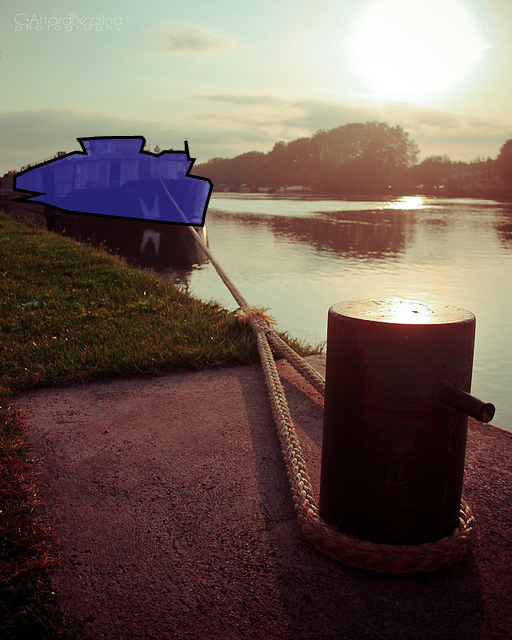
\includegraphics[width=0.7\textwidth]{images/detection.png}
                \caption{Detection example from COCO dataset \cite{lin_microsoft_2015}.}
            \end{figure}
        \end{column}
    \end{columns}
\end{frame}

\begin{frame}{Two types of object detection}
    \begin{figure}
        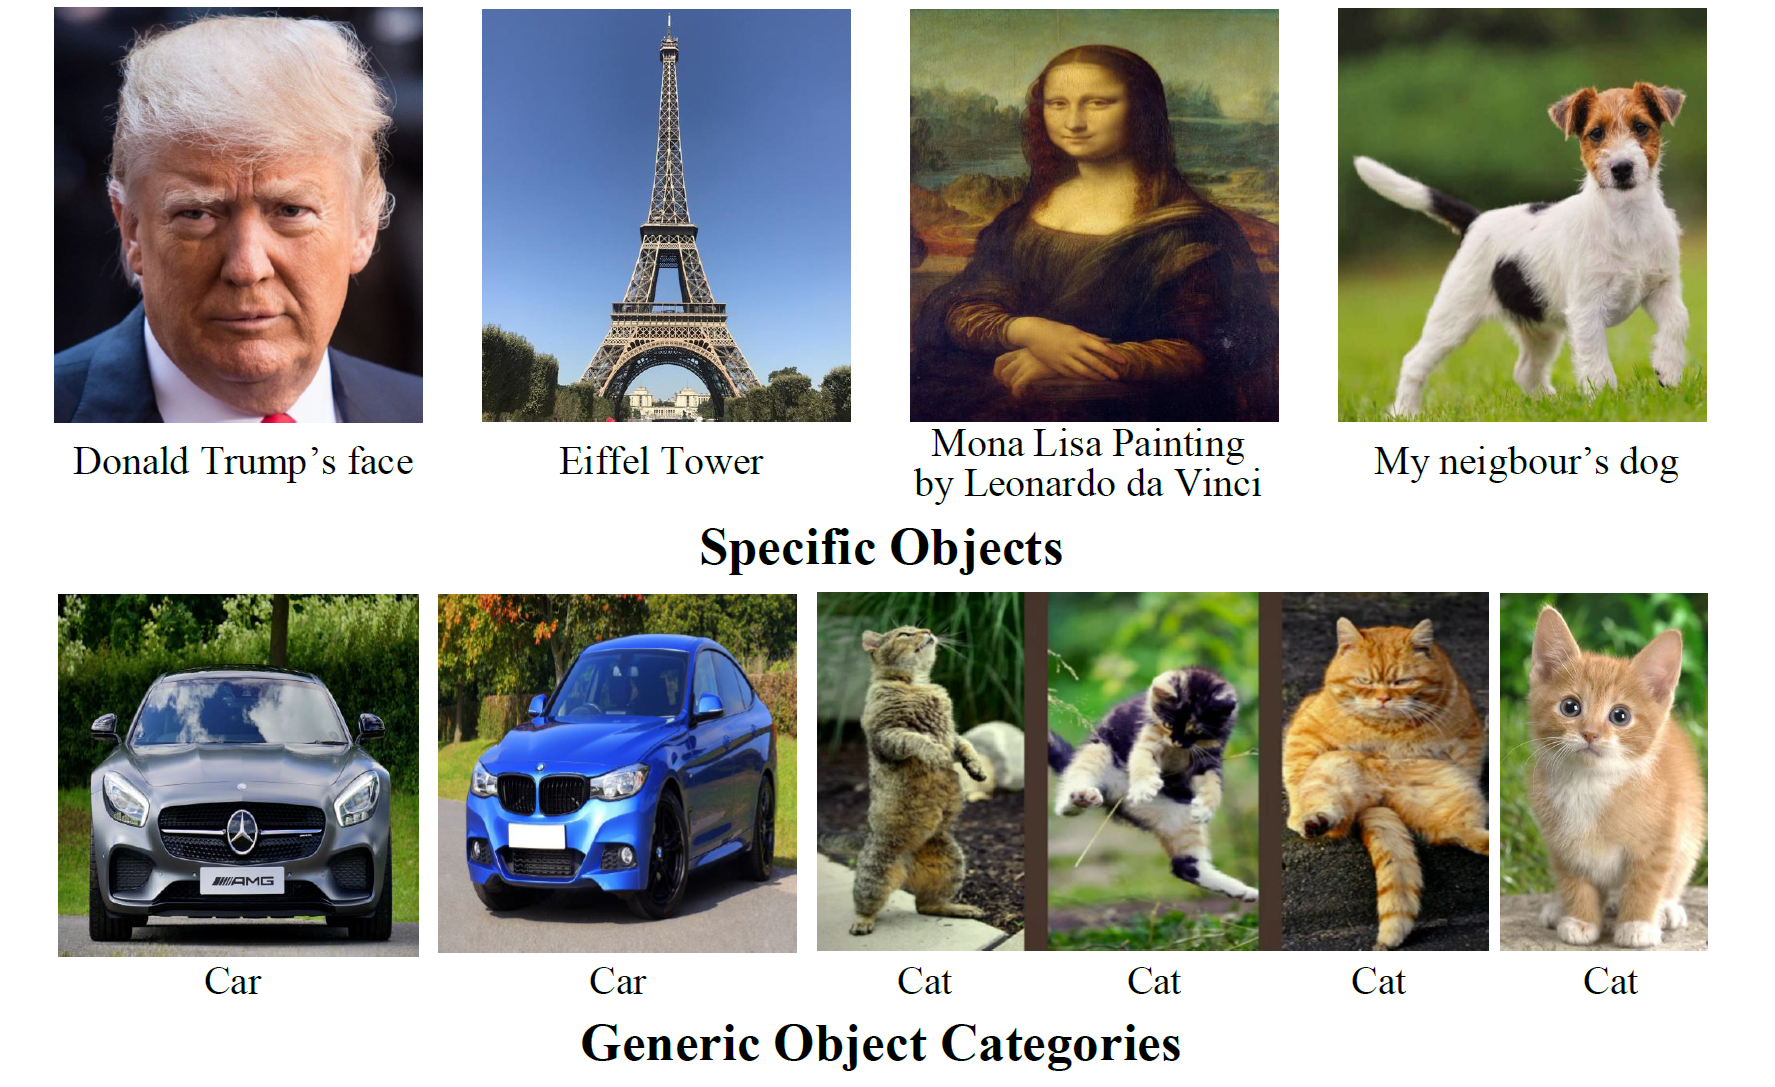
\includegraphics[width=0.8\textwidth]{images/two_types.PNG}
        \caption{Matching \emph{particular} objects versus detecting object \emph{categories} in general.
        \hbox{\scriptsize Credit:\thinspace{\small\itshape \cite{liu_deep_2019}}}
        }
    \end{figure}
\end{frame}

\begin{frame}{The emergence of Deep Learning for Computer Vision}
    \begin{figure}
        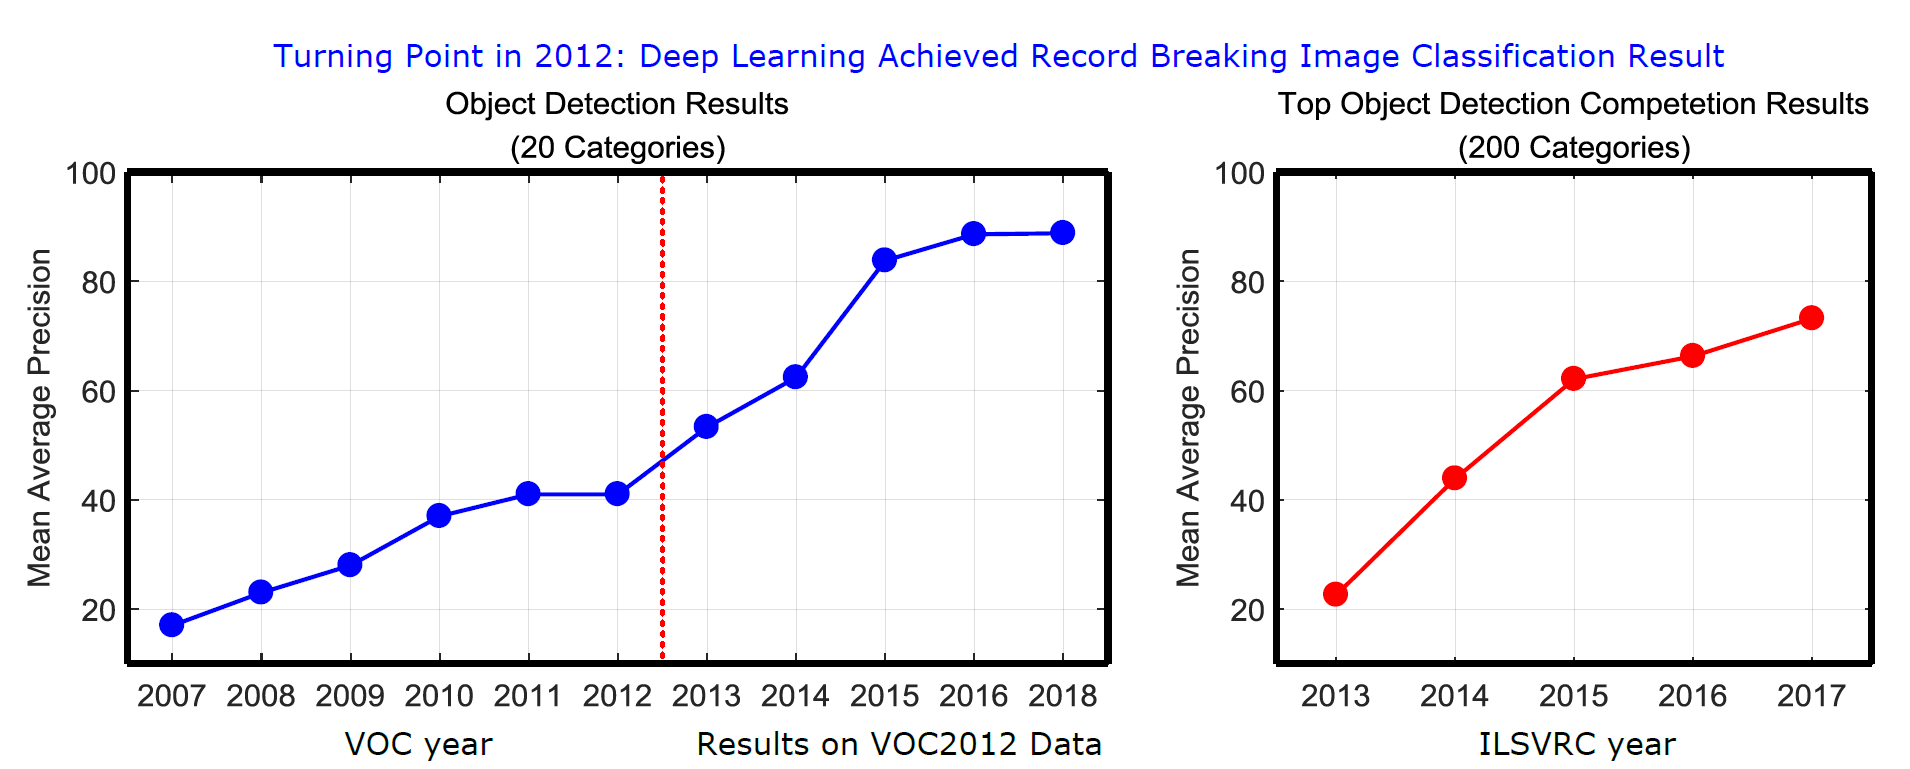
\includegraphics[width=0.9\textwidth]{images/turning_point.PNG}
        \caption{2012 - turning point. \hbox{\scriptsize Credit:\thinspace{\small\itshape \cite{liu_deep_2019}}}}
    \end{figure}
	\begin{itemize}
		\item Detection results of winning entries in the VOC2007-2012 competitions
		\item Top object detection competition results in ILSVRC2013-2017.
	\end{itemize}
\end{frame}

\part{Generic Object Detection}
\begin{frame}
	\partpage
\end{frame}


\section{The Problem}


\begin{frame}{}
    There are many problems closely related to that of generic object detection but we can isolate four main goals.
    \begin{figure}
        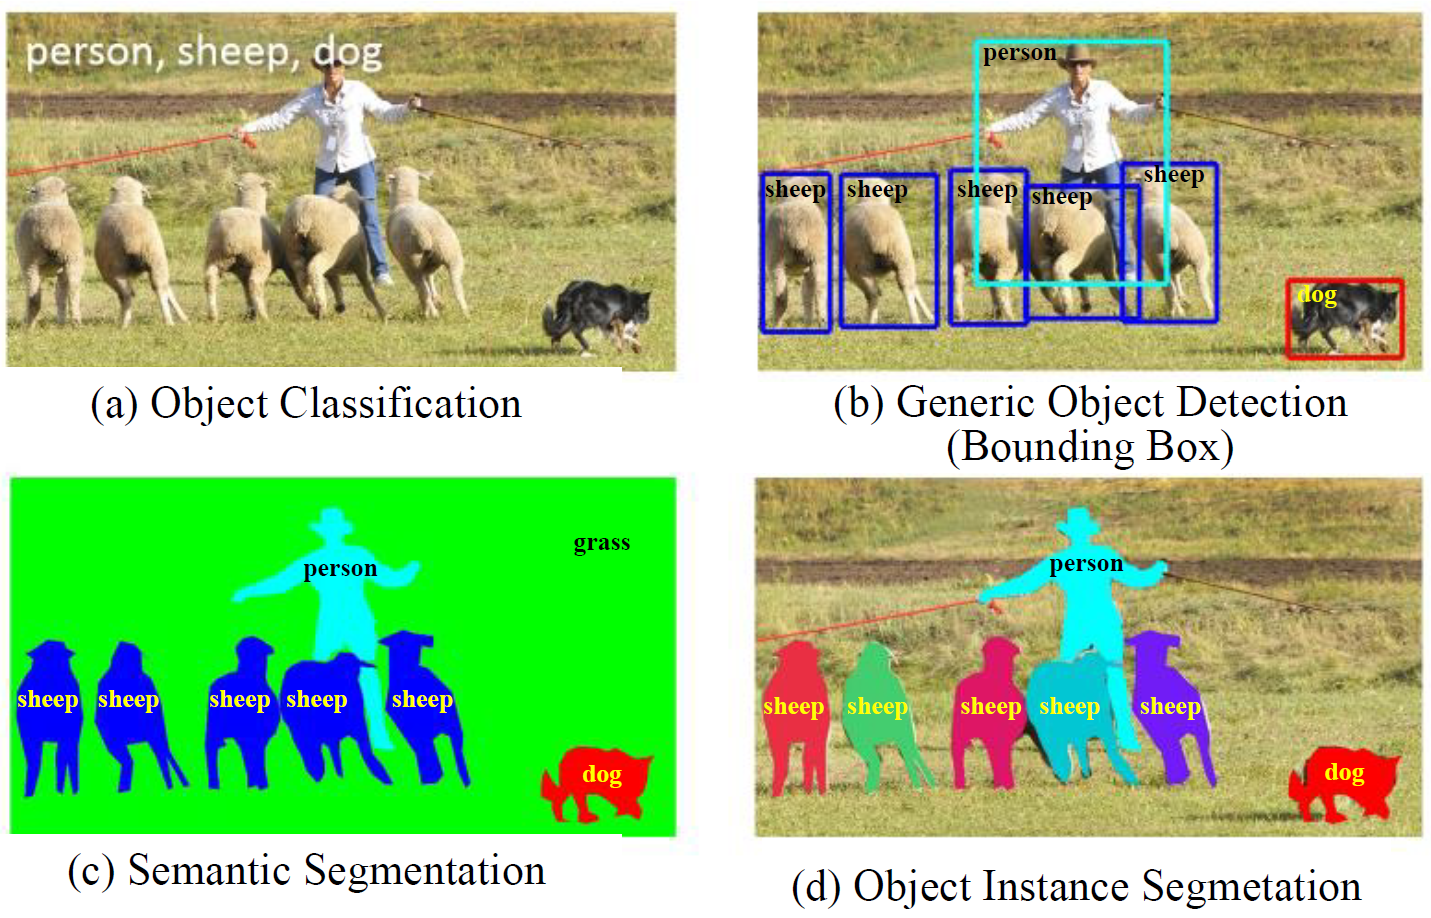
\includegraphics[width=0.7\textwidth]{images/detector_type.PNG}
        \caption{generic object detection
        \hbox{\scriptsize Credit:\thinspace{\small\itshape \cite{liu_deep_2019}}}
        }
    \end{figure}
\end{frame}

\begin{frame}{}
    (a) \emph{object classification}: assess the presence of objects from a given number of object classes in an image.
    \begin{figure}
        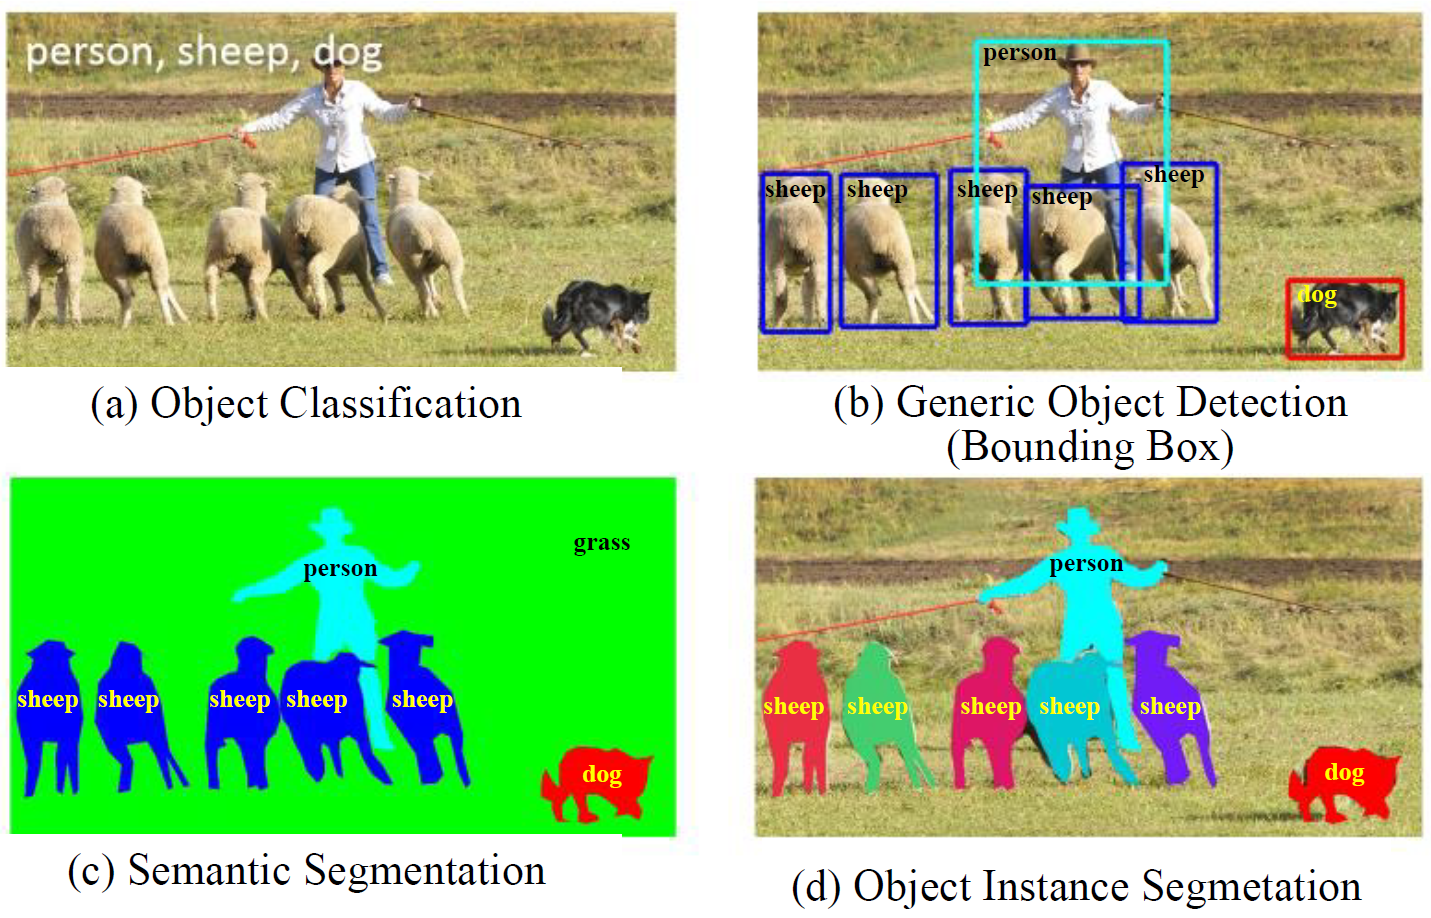
\includegraphics[width=0.7\textwidth]{images/detector_type.PNG}
        \caption{generic object detection
        \hbox{\scriptsize Credit:\thinspace{\small\itshape \cite{liu_deep_2019}}}
        }
    \end{figure}
\end{frame}

\begin{frame}{}
    (b) and (c) \emph{Generic object detection} is closely related to \emph{semantic image segmentation}:  aims to assign each pixel in an image to a semantic class label.
    \begin{figure}
        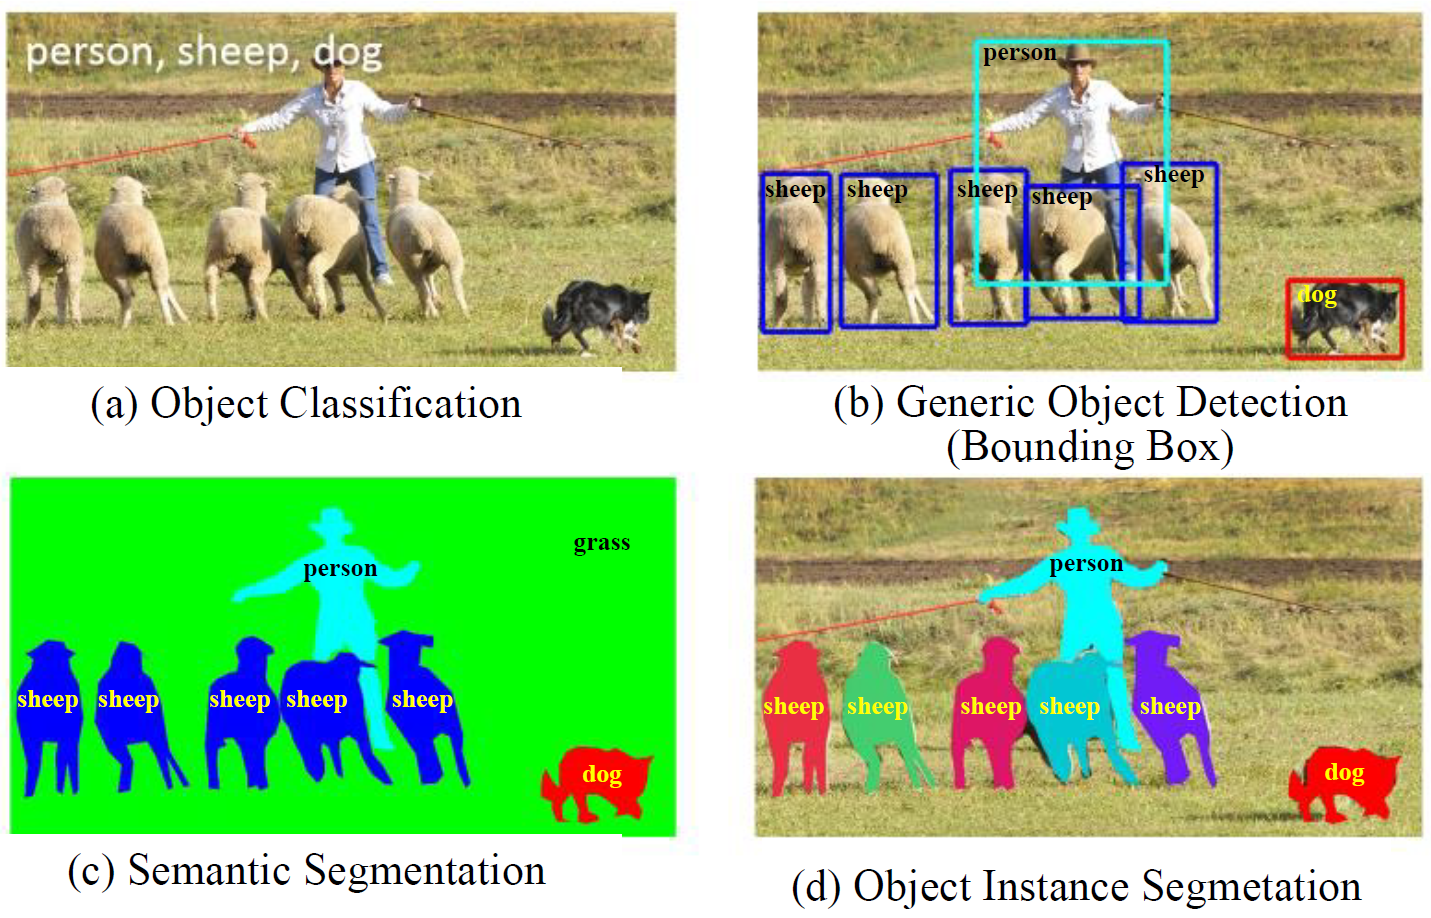
\includegraphics[width=0.7\textwidth]{images/detector_type.PNG}
        \caption{generic object detection
        \hbox{\scriptsize Credit:\thinspace{\small\itshape \cite{liu_deep_2019}}}
        }
    \end{figure}
\end{frame}

\begin{frame}{}
    (d) \emph{Object instance segmentation}: aims to distinguish different instances of the same object class.
    \begin{figure}
        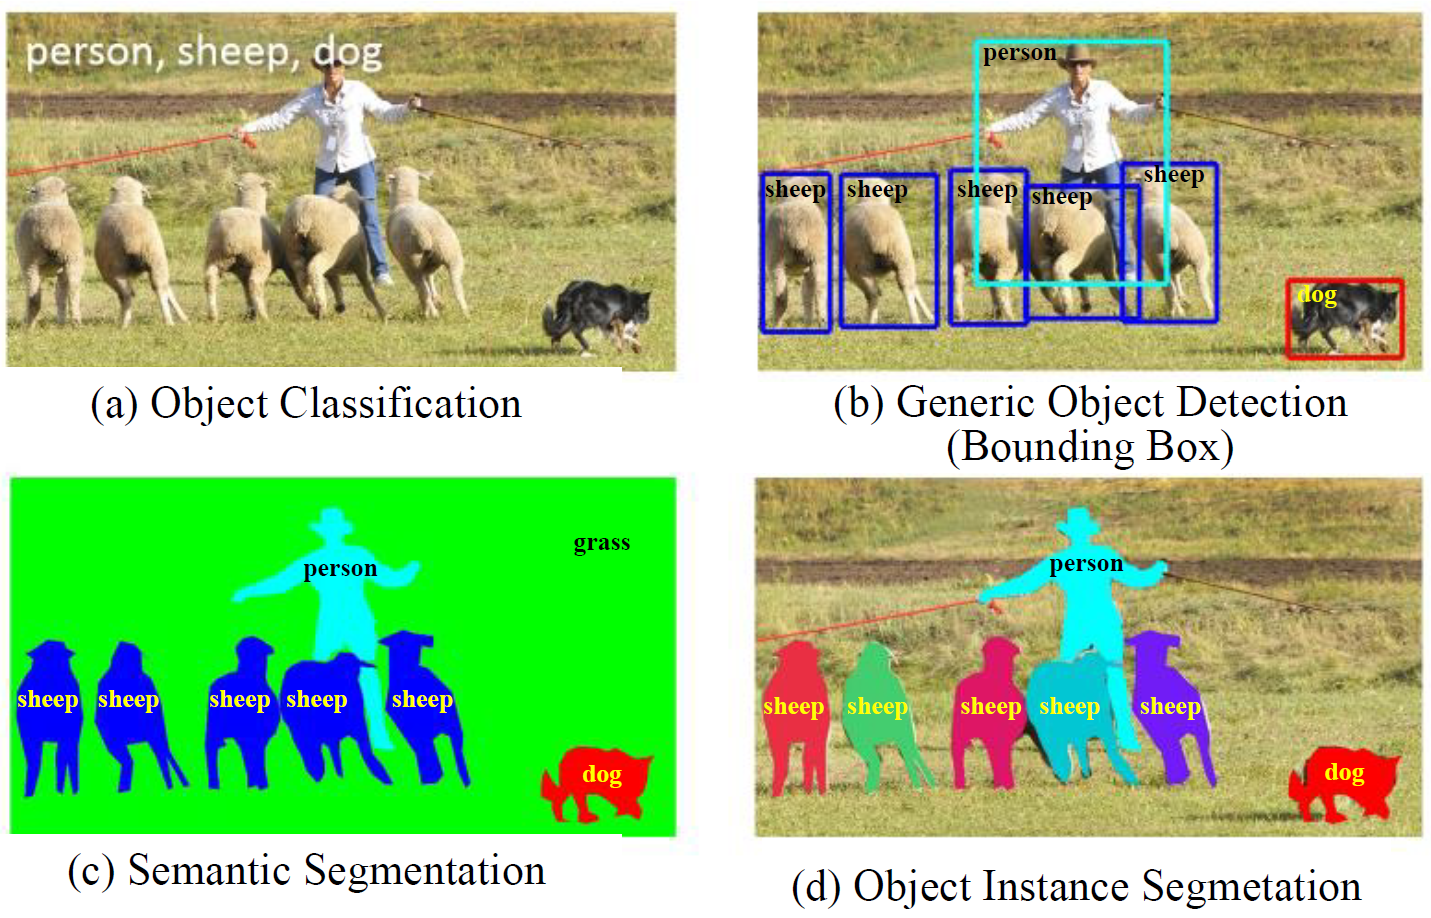
\includegraphics[width=0.7\textwidth]{images/detector_type.PNG}
        \caption{generic object detection
        \hbox{\scriptsize Credit:\thinspace{\small\itshape \cite{liu_deep_2019}}}
        }
    \end{figure}
\end{frame}


\section{Main Challenges}


\begin{frame}
    \begin{columns}
        % Column 1
        \begin{column}{0.45\textwidth}
            \begin{itemize}
                \item \emph{Distinctiveness}: accurately localize and recognize objects in images or video frames.
                \item \emph{Robustness}: object instances from the same category, subject to intra-class appearance variations, can be localized and recognized.
                \item \emph{Efficiency}: entire detection task runs in real time with acceptable memory and storage demands.
            \end{itemize}
        \end{column}
        % Column 2    
        \begin{column}{0.55\textwidth}
            \begin{figure}
                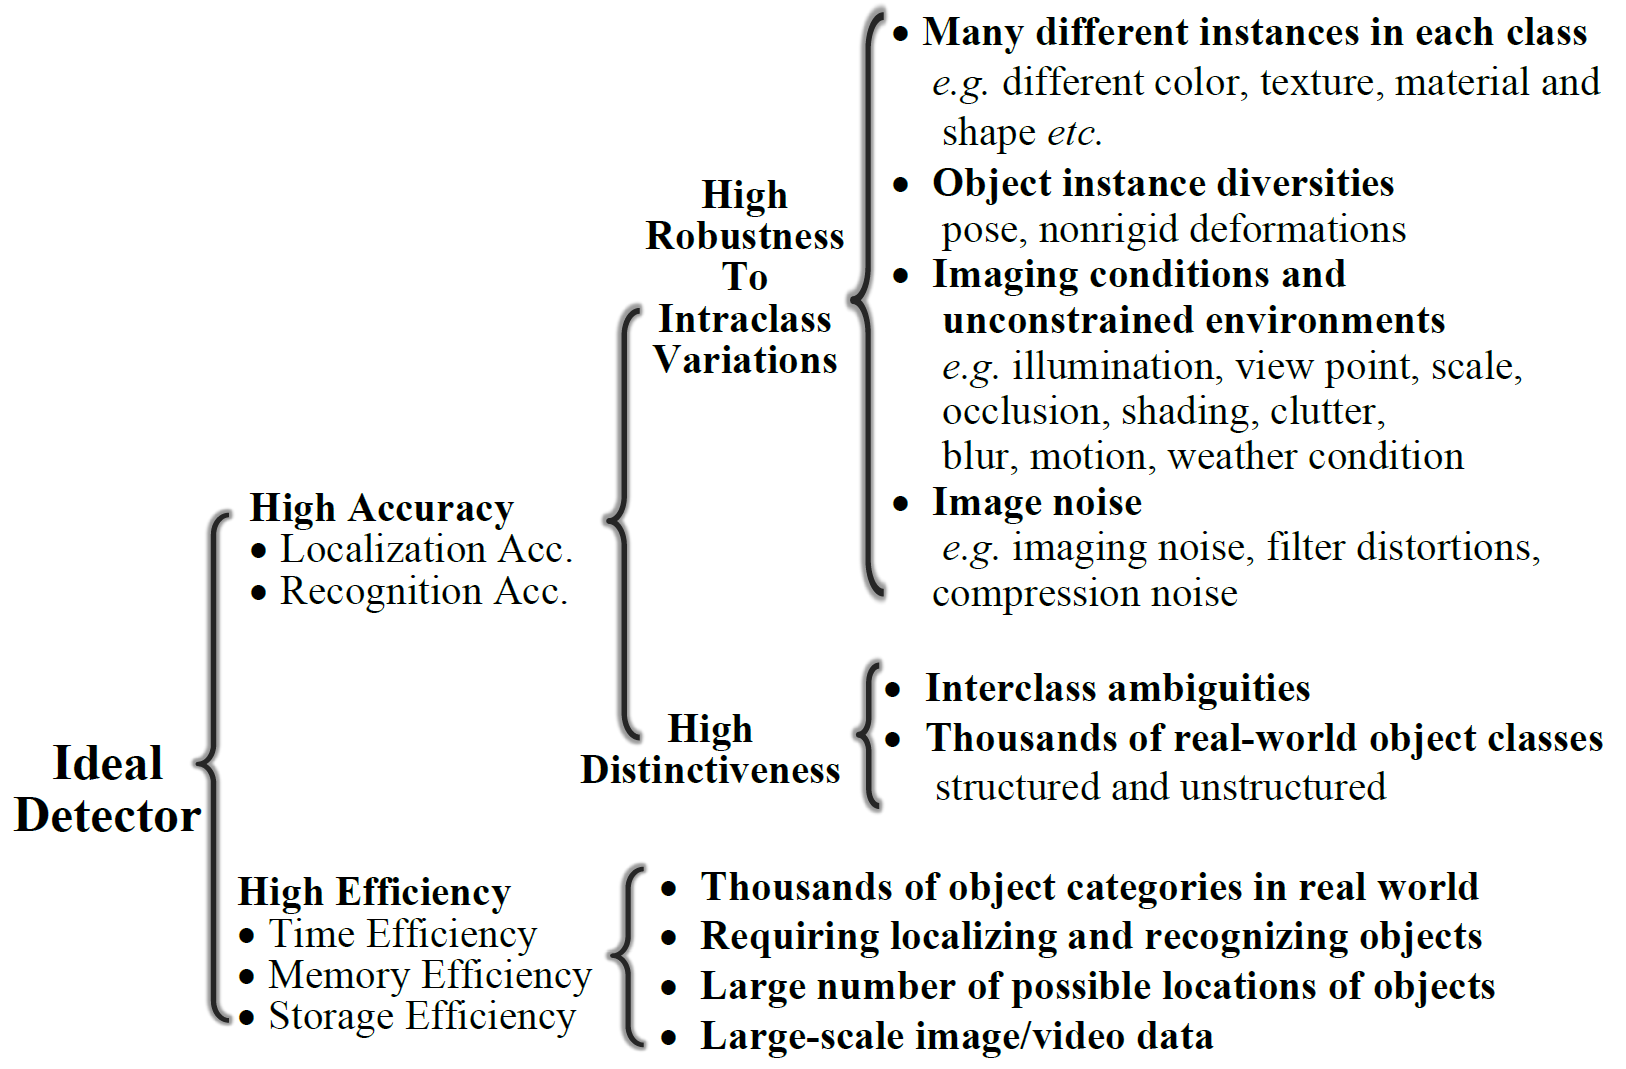
\includegraphics[width=\textwidth]{images/ideal_detector.png}
                \caption{Taxonomy of challenges in generic object detection.
                \hbox{\scriptsize Credit:\thinspace{\small\itshape \cite{liu_deep_2019}}}
                }
            \end{figure}
        \end{column}
    \end{columns}
\end{frame}

\begin{frame}
    \begin{figure}
        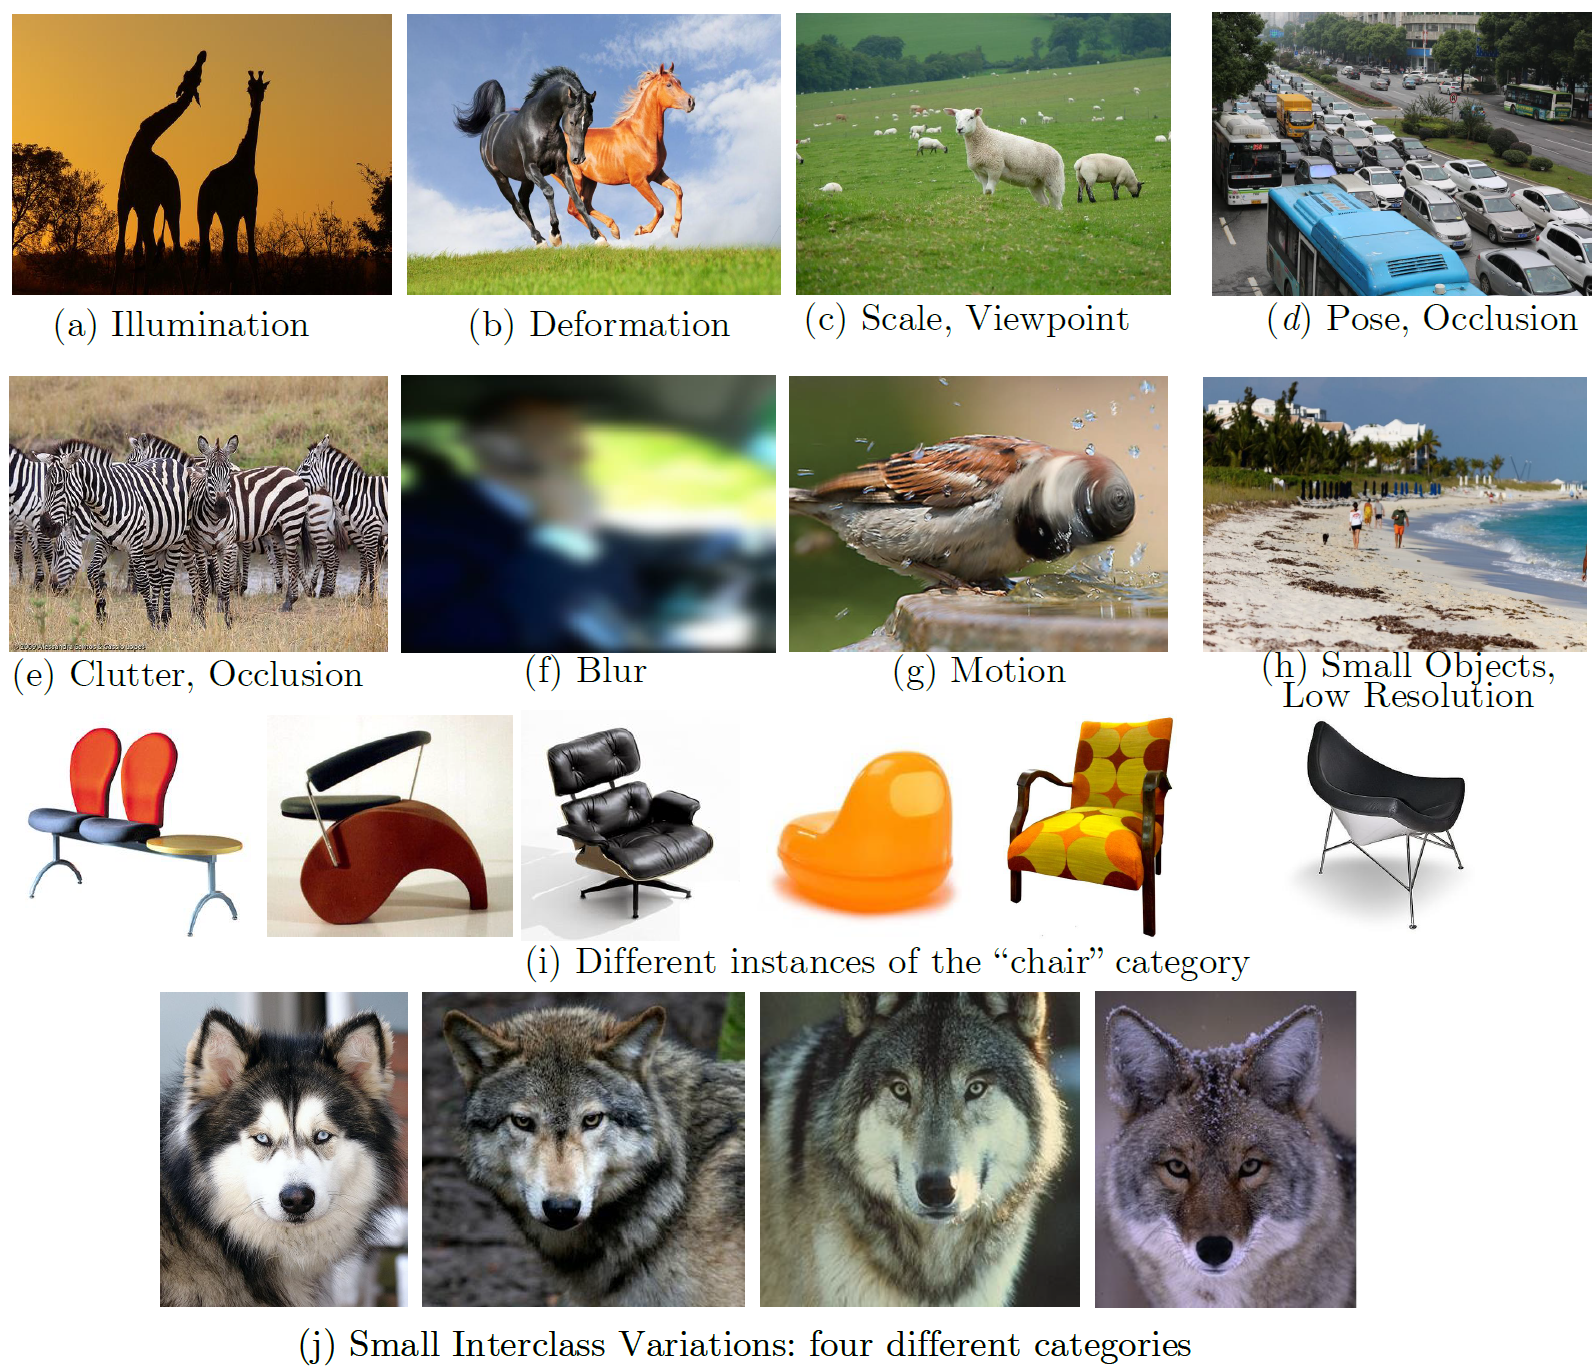
\includegraphics[width=0.65\textwidth]{images/challenge_example.png}
        \caption{(a-j) Intra-class appearance variations. (j) interclasses.
        \hbox{\scriptsize Credit:\thinspace{\small\itshape \cite{liu_deep_2019}}}
        }
    \end{figure}
\end{frame}

\section{Evolution}

%\begin{frame}{}
%    \begin{figure}
%        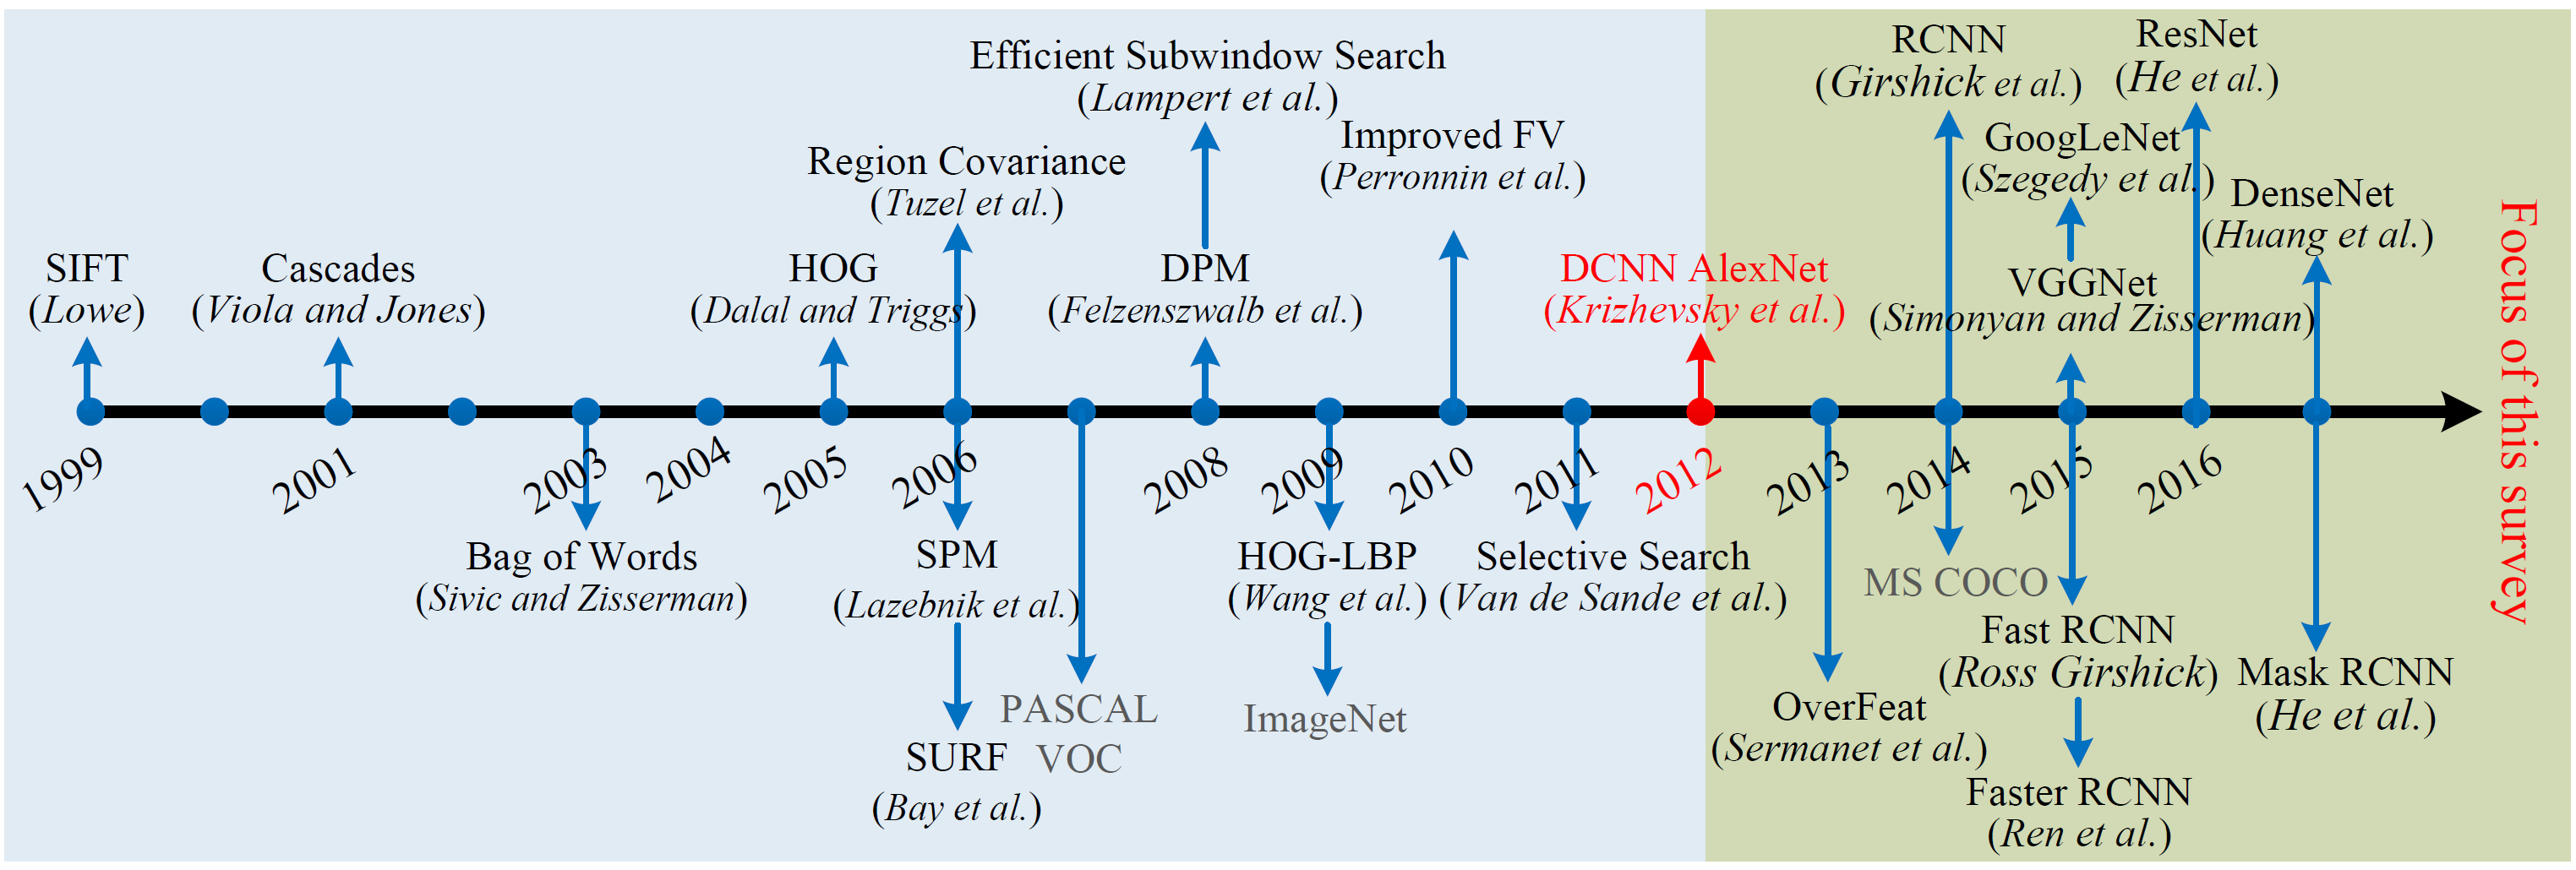
\includegraphics[width=\textwidth]{images/evolution.png}
%        \caption{Evolution of generic object detection framework.
%        \hbox{\scriptsize Credit:\thinspace{\small\itshape  \cite{liu_deep_2019}}}
%        }
%    \end{figure}
%    \begin{itemize}
%        \item 
%        \item Then prior models using statistical classifiers (Neural Networks, SVM, Adaboost) based on appearance features. 
%    \end{itemize}
%\end{frame}

\begin{frame}
    \begin{figure}
        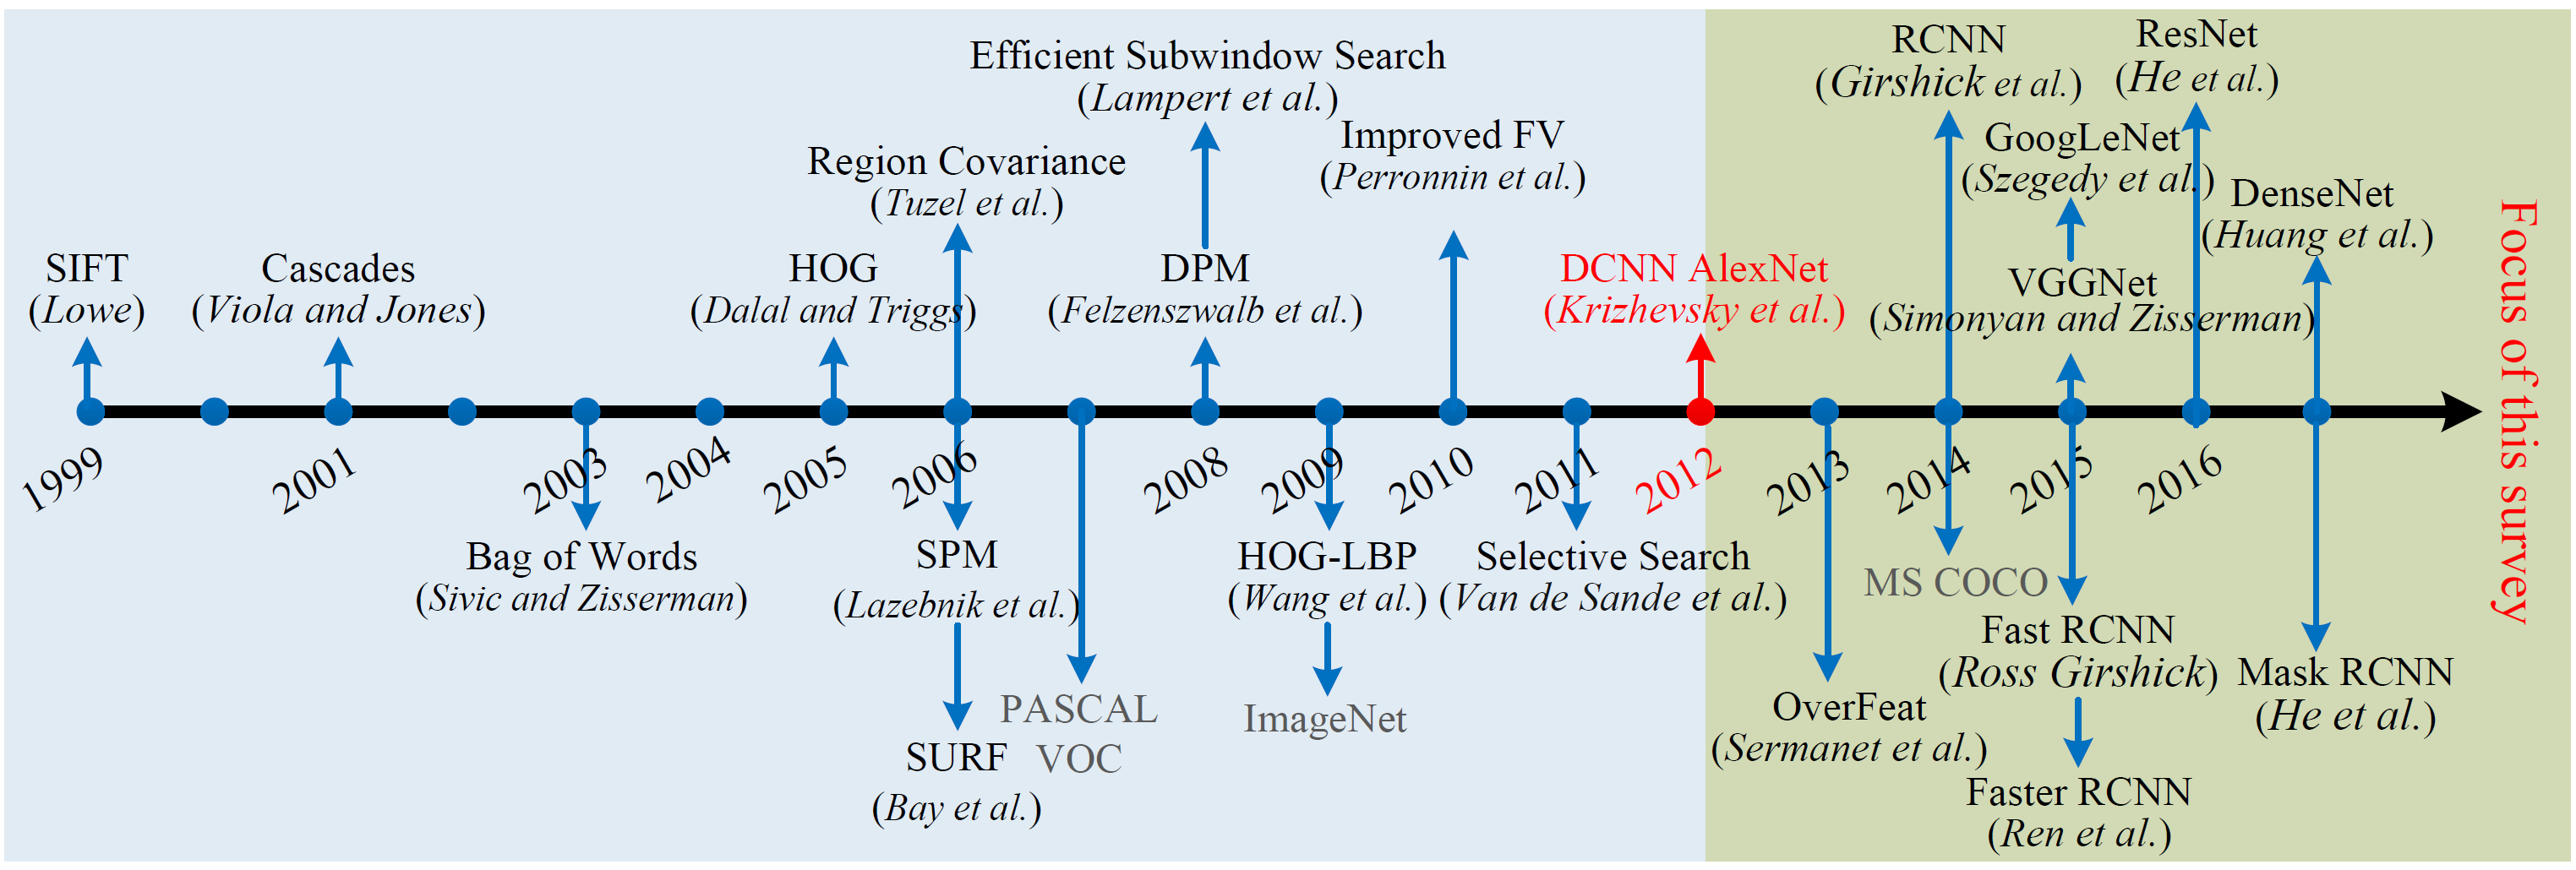
\includegraphics[width=0.8\textwidth]{images/evolution.png}
        \caption{Evolution of generic object detection framework.
        \hbox{\scriptsize Credit:\thinspace{\small\itshape \cite{liu_deep_2019}}}
        }
    \end{figure}
    \begin{itemize}
    	\item Before the 90's leading paradigm based on geometric representations.
        \item Since the 90's two main eras are highlighted, SIFT vs DCNN.
        \begin{itemize}
        	\item Appearance features moved from global to local representations, designed to be invariant to translation, scale, rotation, illumination, viewpoint and occlusion.
        	\item Handcrafted local invariant features gained tremendous popularity, starting from the Scale Invariant and Feature Transform (SIFT).
        \end{itemize}
    \end{itemize}
\end{frame}

\begin{frame}
    \begin{figure}
        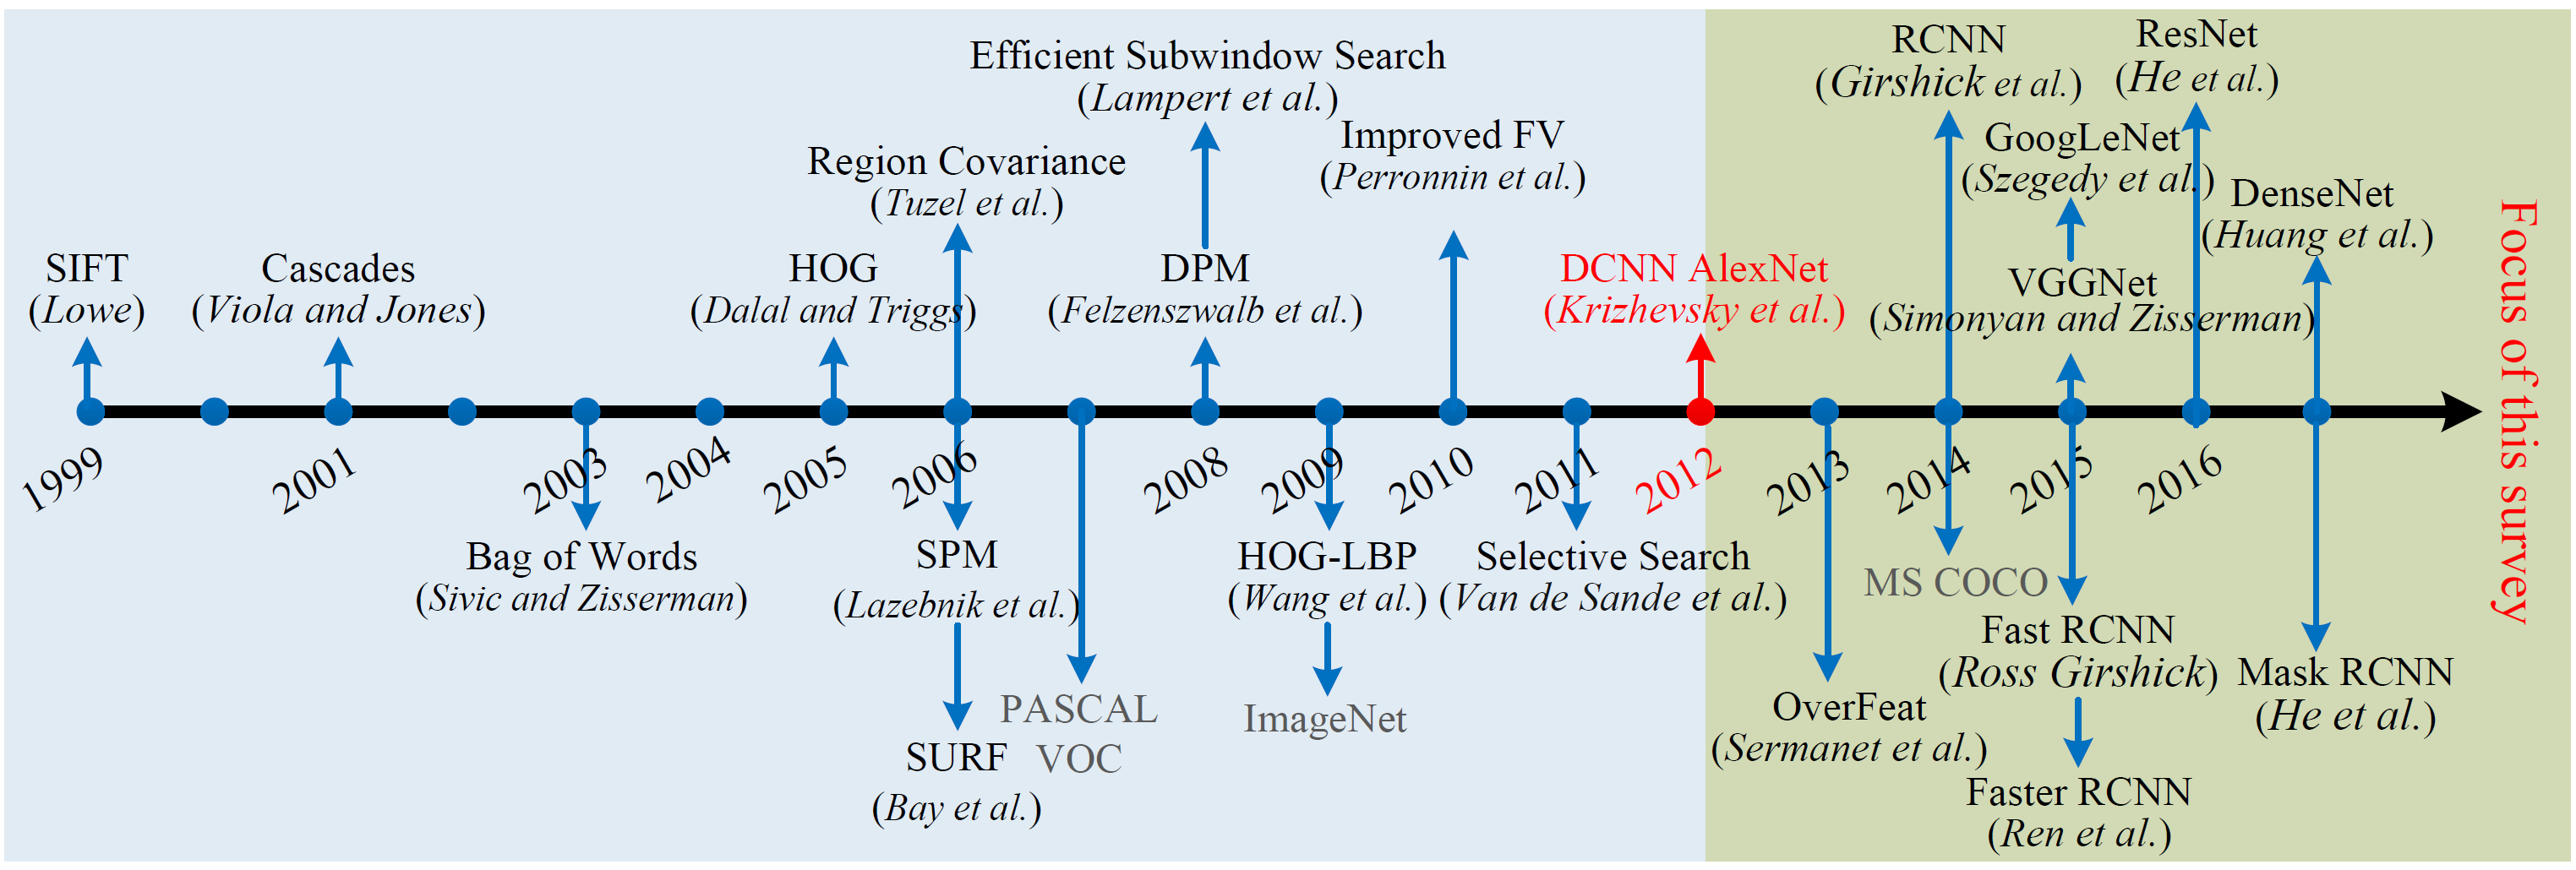
\includegraphics[width=0.8\textwidth]{images/evolution.png}
        \caption{Evolution of generic object detection framework.
        \hbox{\scriptsize Credit:\thinspace{\small\itshape \cite{liu_deep_2019}}}
        }
    \end{figure}
    \begin{itemize}
        \item Significant turning point in 2012 when DCNNs achieved their record-breaking results in image classification.
        \item deeper CNNs have lead to record-breaking improvements in detection of more general object categories, with the milestone Region-based CNN.
        \item Availability of GPUs and large datasets such as ImageNet \cite{russakovsky_imagenet_2015} or MS COCO \cite{lin_microsoft_2015} play a key role in their success.
    \end{itemize}
\end{frame}


\part{Datasets and Performance Evaluation}
\begin{frame}
	\partpage
\end{frame}


\section{Datasets}


\begin{frame}
    Four famous large high quality datasets set milestones: PASCAL VOC \cite{everingham_pascal_2010}, ImageNet \cite{krizhevsky_imagenet_2017}, MS COCO \cite{lin_microsoft_2015} and Open Images \cite{kuznetsova_open_2020}. For creating large-scale annotated datasets:
    \begin{enumerate}
        \item determining the set of target object categories,
        \item collecting a diverse set of candidate images to represent the selected categories on the Internet,
        \item annotating the large amount of collected images, typically by designing crowdsourcing strategy.
    \end{enumerate}
    The four datasets form the backbone of their respective detection challenges. Each challenge consists of a publicly available dataset of images together with ground truth annotation and standardized evaluation software, and an annual competition and corresponding workshop.
\end{frame}

\begin{frame}
	\begin{figure}
		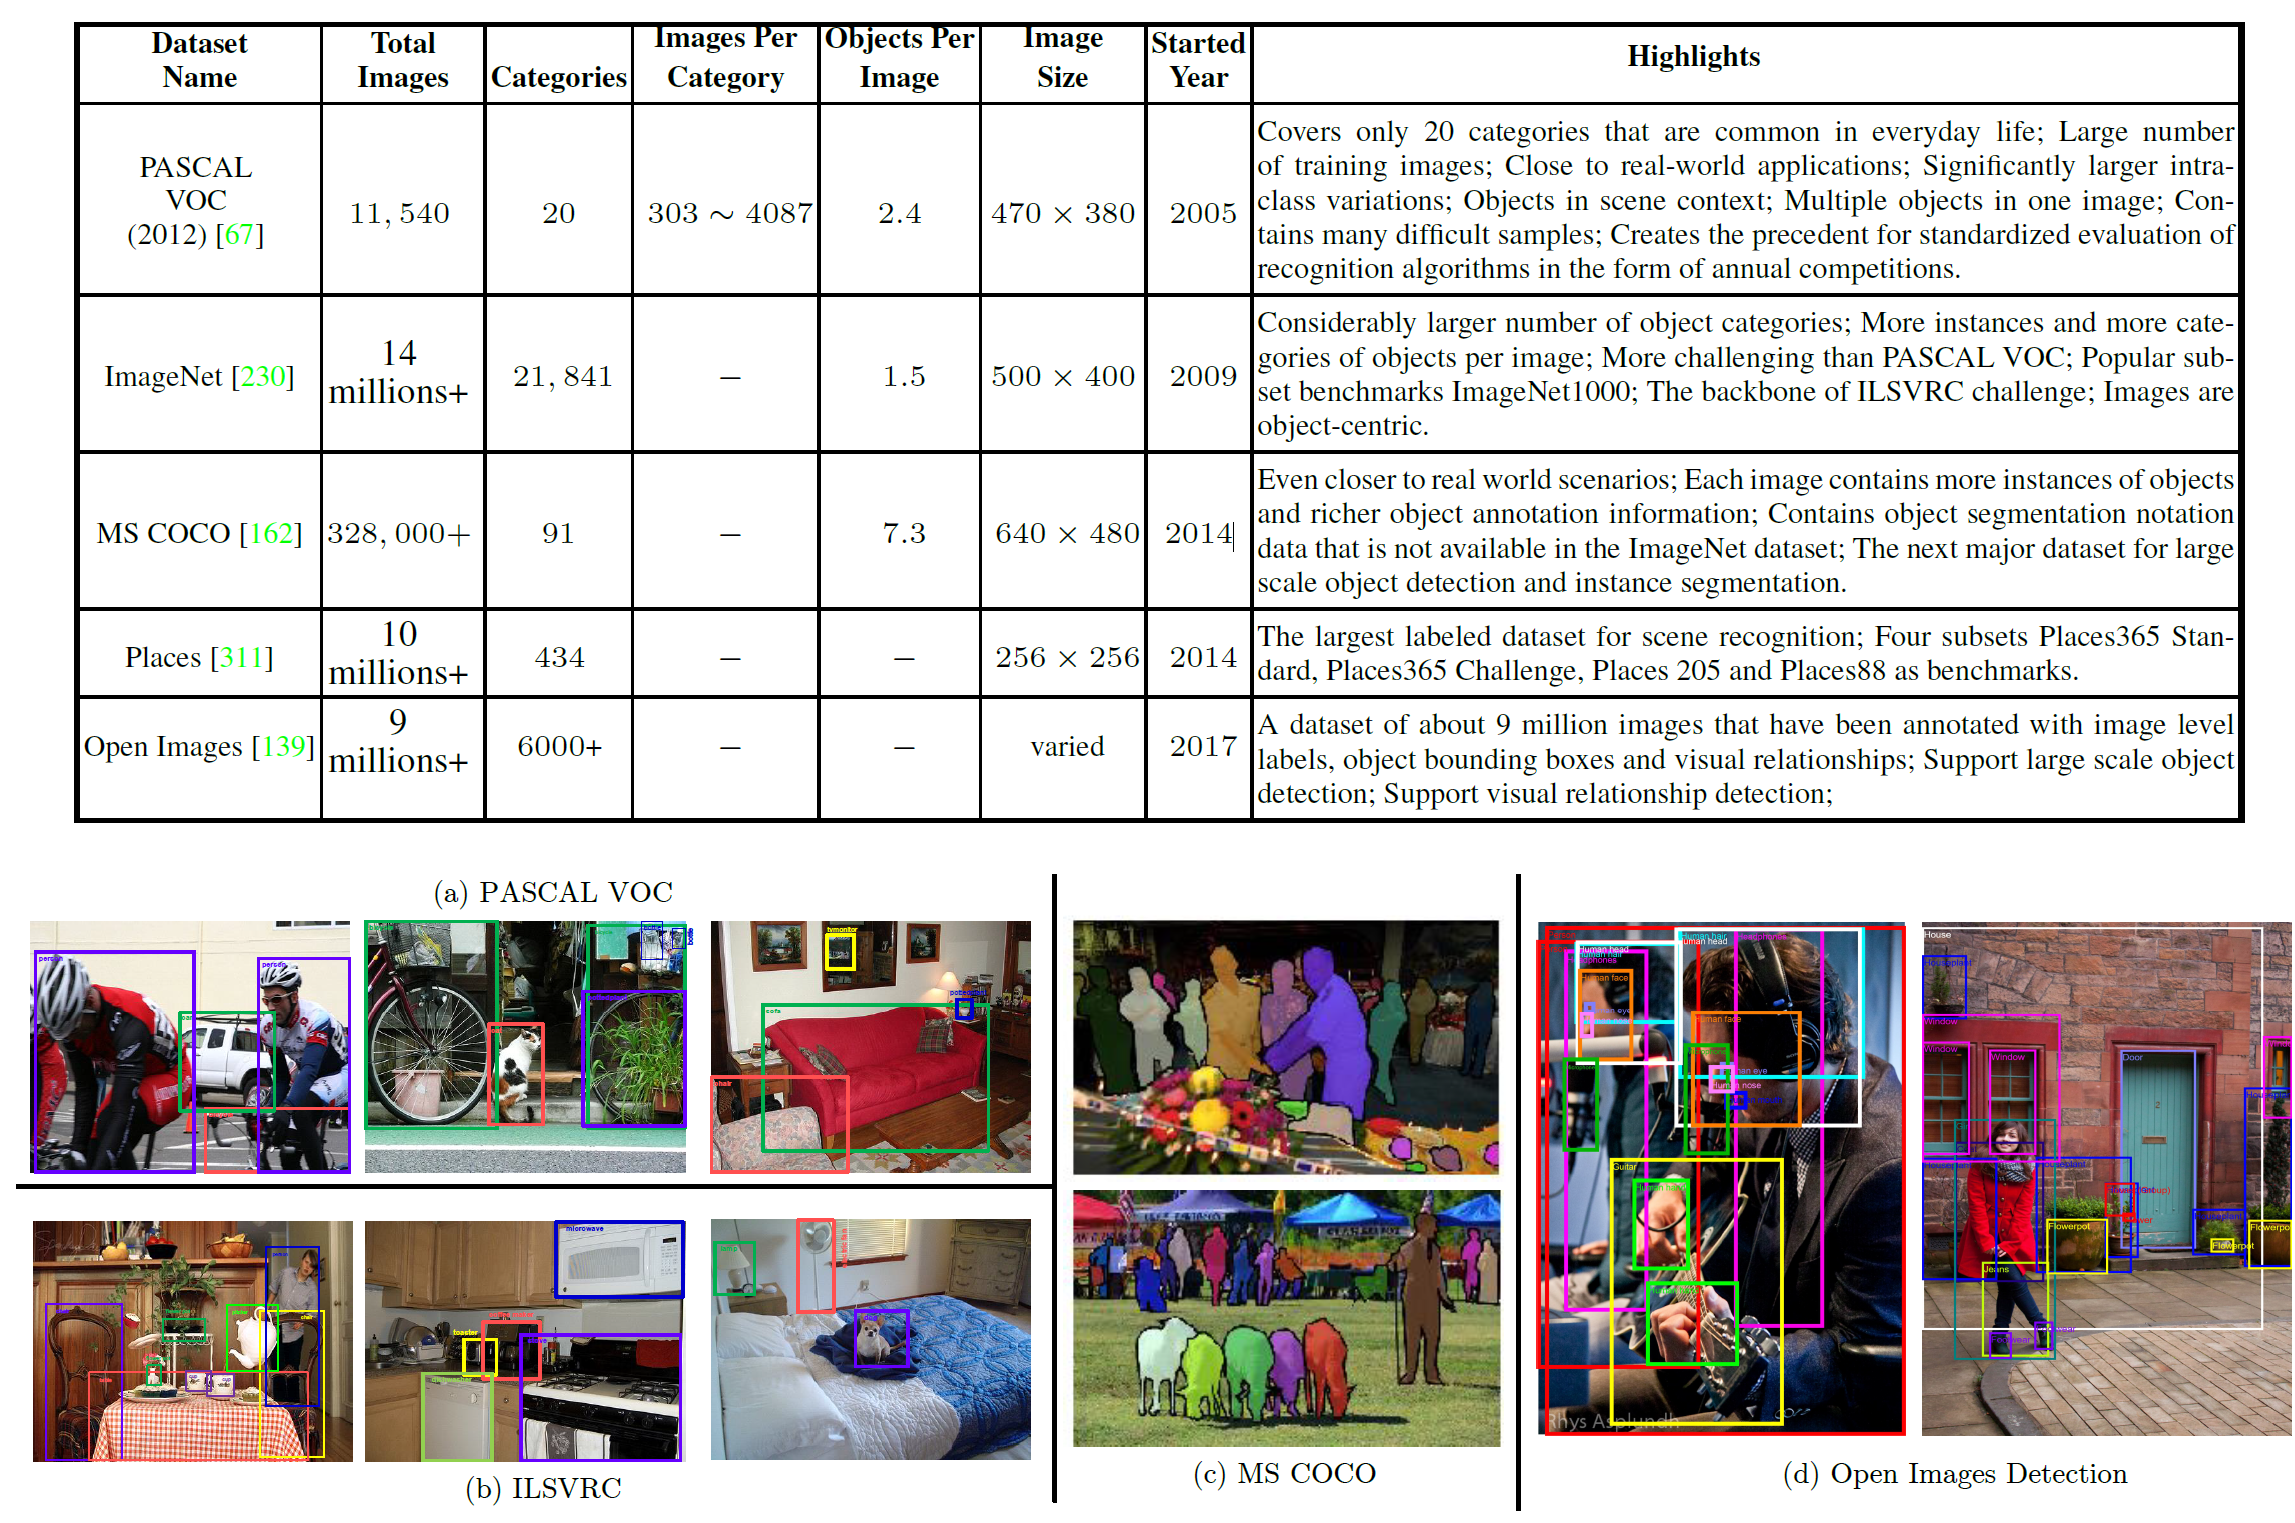
\includegraphics[width=\textwidth]{images/datasets.png}
        \caption{Main available datasets.
        \hbox{\scriptsize Credit:\thinspace{\small\itshape \cite{liu_deep_2019}}}
        }
    \end{figure}
\end{frame}

\begin{frame}{Question}
	Your boss ask you to train an algorithm able to detect saiboats at sea.
	What is your first idea for creating a train set ?
\end{frame}


\section{Evaluation Criteria}


\begin{frame}
	Evaluating the performance of detection algorithms:
    \begin{itemize}
        \item Detection speed in Frame Per Second (FPS)
        \item $Precision = \frac{TP}{TP + FP}$ - What proportion of positive identifications was actually correct?
        \item $Recall = \frac{TP}{TP + FN}$ - What proportion of actual positives was identified correctly?
    \end{itemize}
	The standard outputs of a detector applied to a testing image $I$ are the predicted detections $\{(b_j ; c_j ; p_j)\}_j$ , indexed by $j$ and denotes
	\begin{itemize}
		\item the predicted location (i.e., the Bounding Box, BB) $b$,
		\item its predicted category label $c$,
		\item its confidence level $p$.
	\end{itemize}
\end{frame}

\begin{frame}
	\begin{figure}
		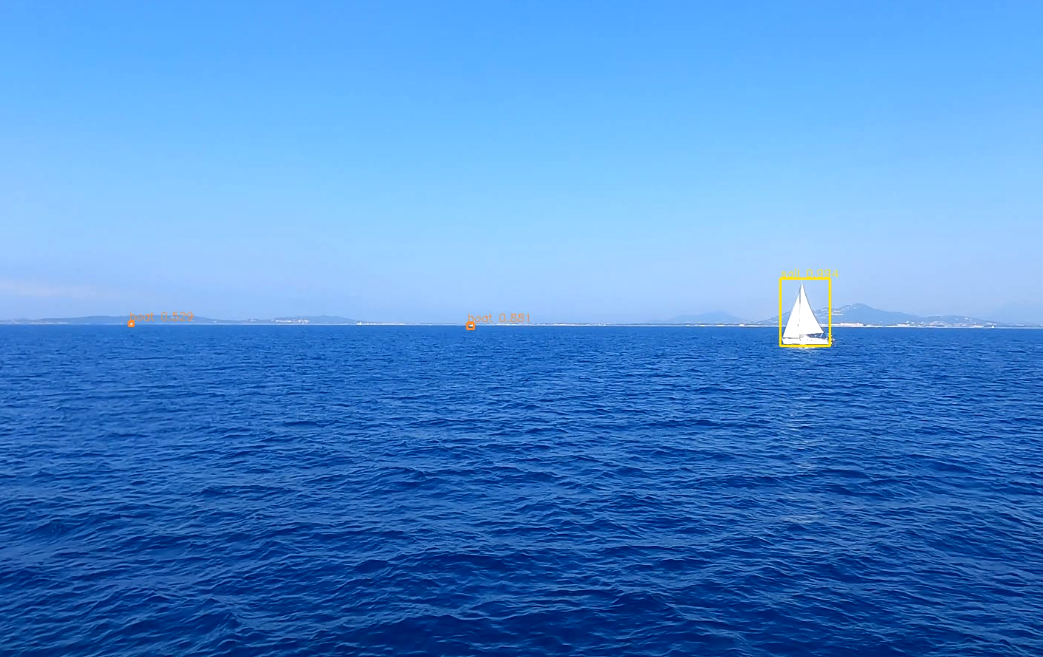
\includegraphics[width=\textwidth]{images/detection_example.png}
		\caption{Example of a detection.
			\hbox{\scriptsize Credit:\thinspace{\small\itshape Eca Robotics}}
		}
	\end{figure}
\end{frame}


\subsection{Intersection Over Union}
\begin{frame}{}
	\begin{columns}
		% Column 1
		\begin{column}{0.6\textwidth}
			A predicted detection $(b; c; p)$ is TP if
			\begin{itemize}
				\item The predicted category label $c$ == the ground truth label $c_g$ i.e. if $p > \epsilon$, where $\epsilon$ is a chosen threshold.
				\item The overlap ratio Intersection Over Union $IOU(b, b^g) = \frac{area(b \cap b^g)}{area(b \cup b^g)} > \beta$, typically 0.5.
			\end{itemize}
			Otherwise, it is considered as FP.
		\end{column}
		\begin{column}{0.4\textwidth}
			\begin{figure}
				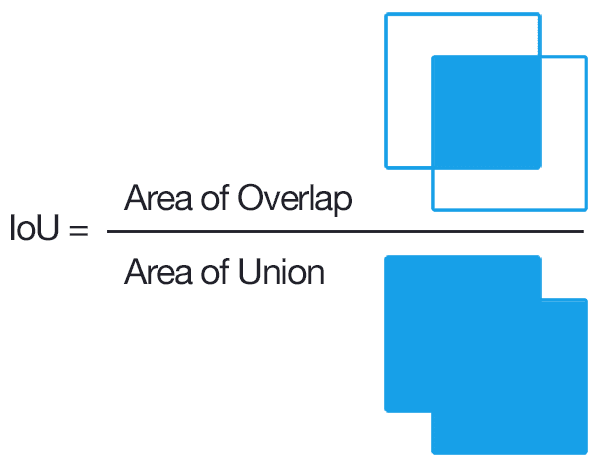
\includegraphics[width=\textwidth]{images/IOU.PNG}
				\caption{IoU formula}
			\end{figure}
		\end{column}
	\end{columns}
\end{frame}


%\begin{frame}{Intersection Over Union}
%	\begin{figure}
%		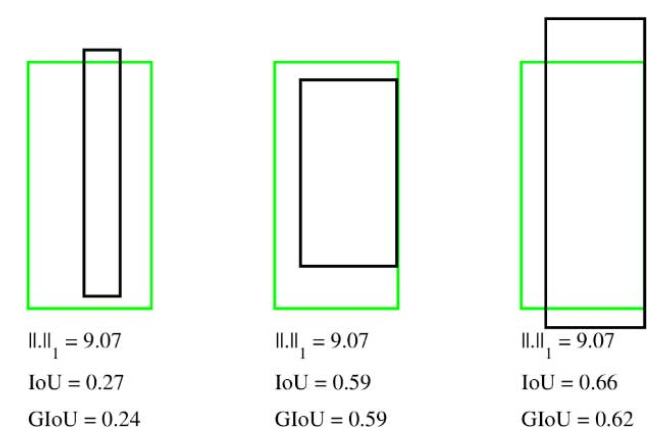
\includegraphics[width=0.7\textwidth]{images/GIOU.PNG}
%		\caption{Examples of IOU calculus.
%			\hbox{\scriptsize Credit:https://giou.stanford.edu/}
%		}
%	\end{figure}
%\end{frame}


\subsection{Precision-Recall Curve}
\begin{frame}{}
	\begin{columns}
		% Column 1
		\begin{column}{0.6\textwidth}
			\begin{itemize}
				\item Precision-recall curve the shows the tradeoff between the precision and recall values for different thresholds, here $\beta$.
				\item Helps to select the best threshold to maximize both metrics.
				\item For creating that curve you need:
				\begin{itemize}
					\item the ground-truth labels,
					\item the prediction scores of the samples,
					\item some thresholds to convert the prediction scores into class labels.
				\end{itemize}
			\end{itemize}
		\end{column}
		\begin{column}{0.4\textwidth}
			\begin{figure}
				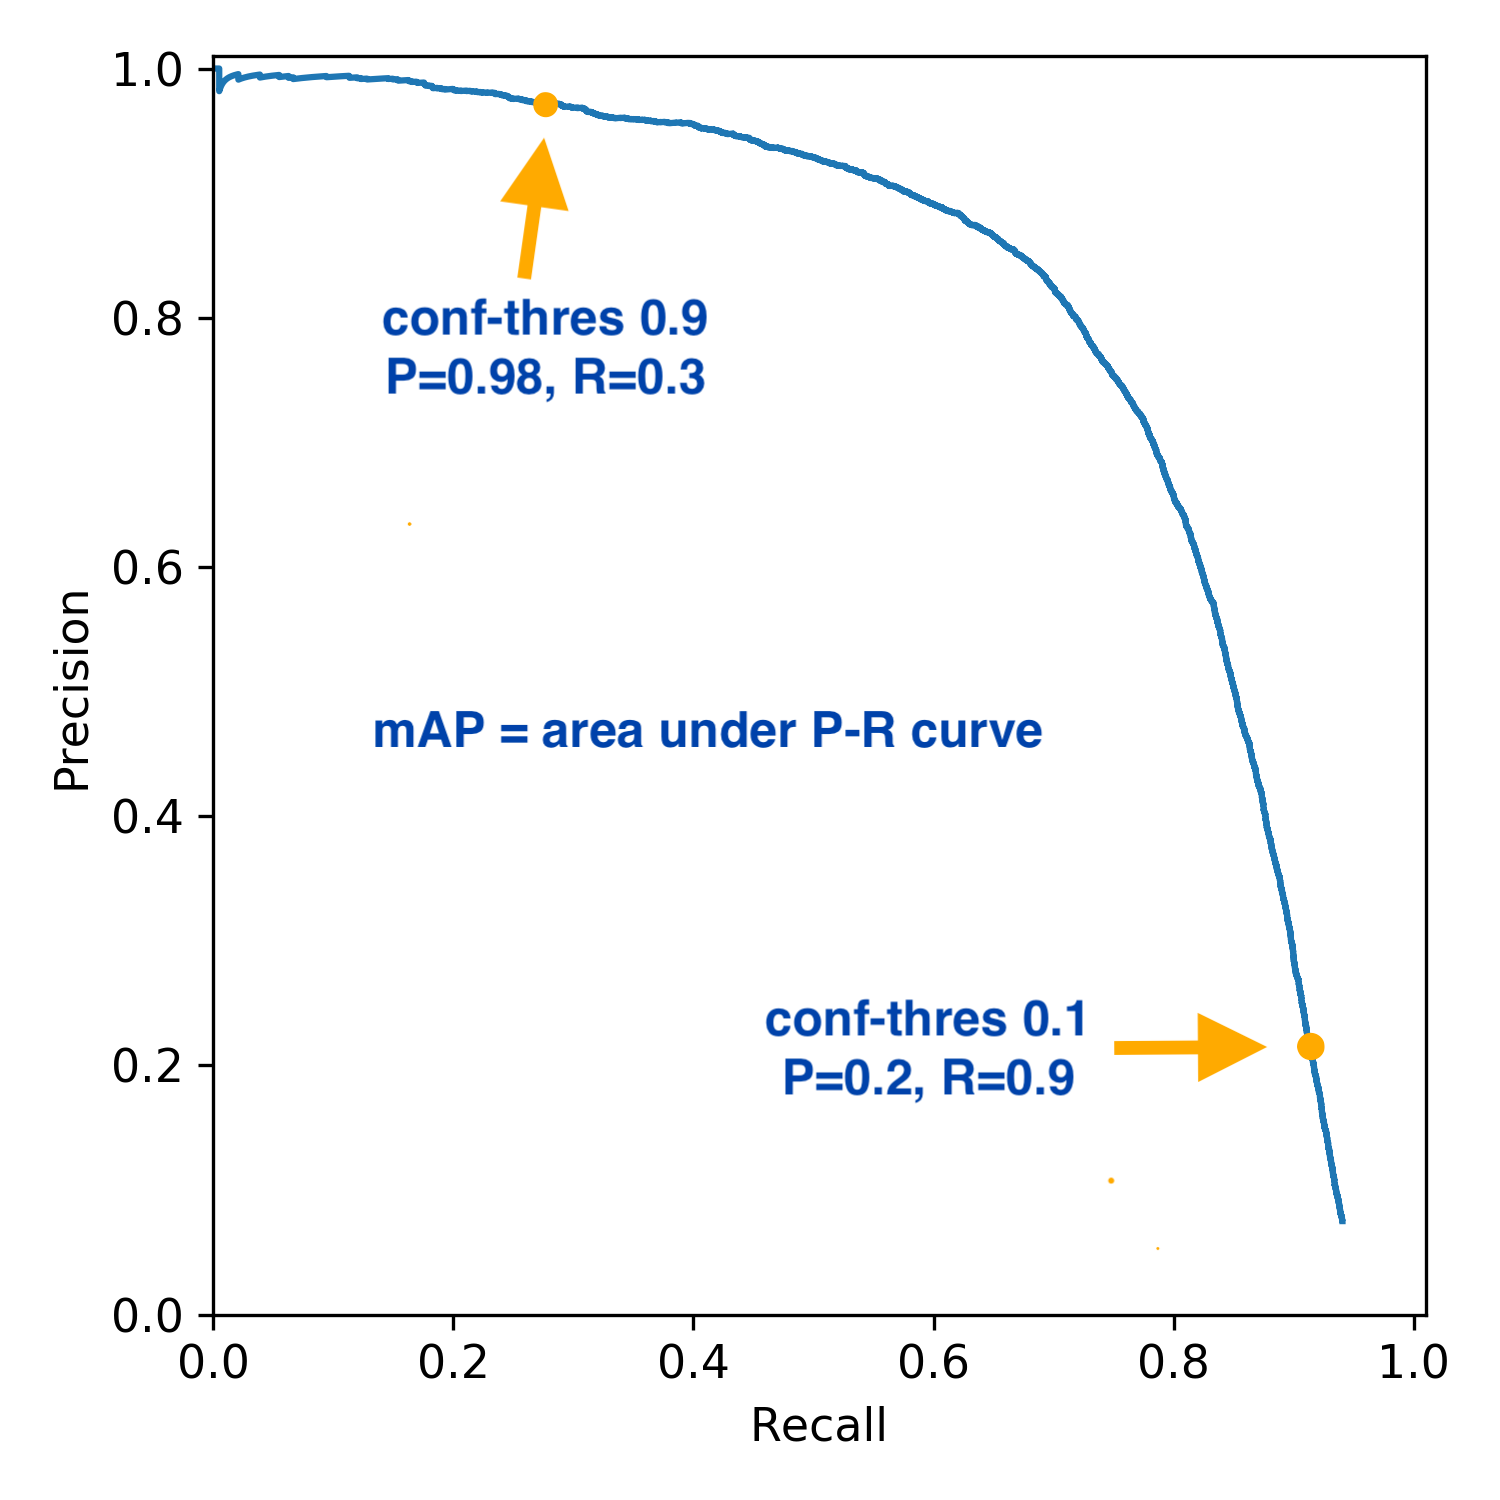
\includegraphics[width=\textwidth]{images/precision_recall.png}
				\caption{Precision-recall curve example}
			\end{figure}
		\end{column}
	\end{columns}
\end{frame}


\subsection{Average Precision}
\begin{frame}{}
	The most commonly used metric is \emph{Average Precision} (AP), derived from precision and recall and computed by class.
    \begin{enumerate}
        \item For a given class $c$ and a testing image $I$, let ${(b_{j} ; p_{j})}^M_{j=1}$ denote the detections returned by a detector, ranked by the confidence $p_{j}$ in decreasing order.
        % \item Let $\mathcal{B}  = {b^g_{ik}}^K_{k=1}$ be the ground truth boxes on image $I_i$, for the given object class c.
        \item Each detection $(b_{j} ; p_{j})$ is either a TP or a FP using IoU calculus.
        \item Based on the TP and FP detections, the precision $P(\beta)$ and recall $R(\beta)$ can be computed as a function of IoU threshold $\beta$.
        \item Finally AP is a sum of the increases on recall weighted by the precision.
        \item For example for thresholds $\beta \in \{0.5,..,0.9\}$,  $$AP = \sum_{\beta=0.5}^{0.9}(R(\beta) - R(\beta+1)) * P(\beta)$$, with $R(0) = 0$ and $P(1)=1$
    \end{enumerate}
\end{frame}

\begin{frame}{}
	\begin{columns}
		% Column 1
		\begin{column}{0.6\textwidth}
			\begin{itemize}
				\item AP is a way to summarize the precision-recall curve into a single value representing the average of all precisions.
				\item It is the weighted sum of precisions at each threshold where the weight is the increase in recall.
				\item Question: Could you imagine a single metric for evaluating object detector on a whole dataset ?
			\end{itemize}
		\end{column}
		\begin{column}{0.4\textwidth}
			\begin{figure}
				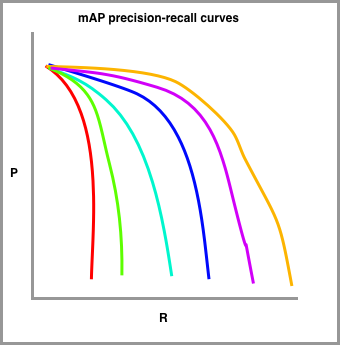
\includegraphics[width=\textwidth]{images/AP.png}
				\caption{Average Precision}
			\end{figure}
		\end{column} 
	\end{columns}
\end{frame}


\subsection{Mean Average Precision - mAP}
\begin{frame}{}
	\begin{columns}
		% Column 1
		\begin{column}{0.5\textwidth}
			\begin{itemize}
				\item Object detection models are evaluated with different IoU thresholds where each threshold may give different predictions from the other thresholds.
				\item For example for COCO: $IoU=.50:.05:.95$
				\item $$ mAP = \frac{1}{n} \sum_{k=1}^{n} AP_k $$, where $AP_k$ is the $AP$ of class $k$ and $n$ is the number of classes.
			\end{itemize}
		\end{column}
		\begin{column}{0.5\textwidth}
			\begin{figure}
				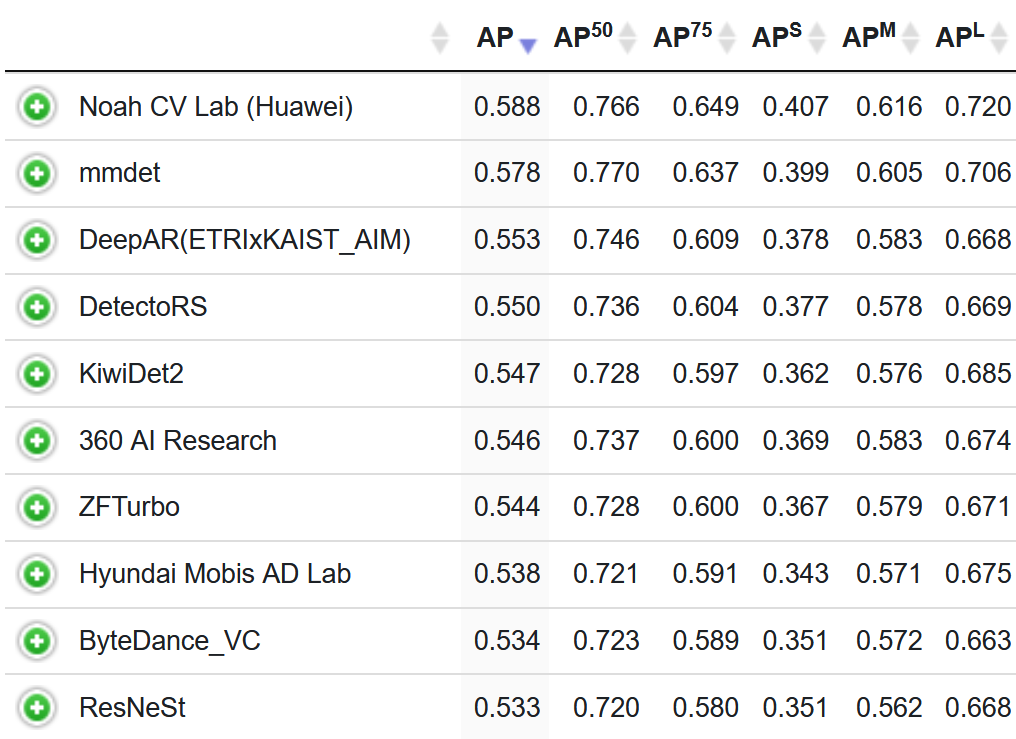
\includegraphics[width=\textwidth]{images/coco_leaderboard.png}
				\caption{Average Precision on COCO detection leaderboard}
			\end{figure}
		\end{column} 
	\end{columns}
\end{frame}

% For the practical work
% In your opinion Always same AP for all sizes ?
% How could you know ?


\part{Detection frameworks}
\begin{frame}
	\partpage
\end{frame}


\begin{frame}
	Detectors organized into two main categories:
	\begin{enumerate}
		\item Two stage detection framework, which includes
			\begin{enumerate}
				\item region proposal,
				\item objects classification and localization.
			\end{enumerate}
		\item One stage detection framework, or region proposal free framework, which is method to propose region, classify and localize objects in a single step.
	\end{enumerate}
	\begin{figure}
		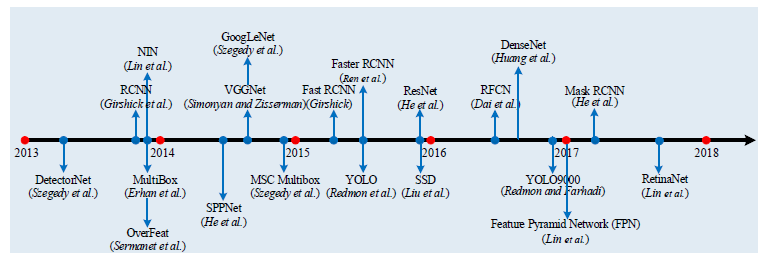
\includegraphics[width=0.9\textwidth]{images/detection_framework.PNG}
		\caption{Milestones of object detection frameworks
			\hbox{\scriptsize Credit:\thinspace{\small\itshape \cite{liu_deep_2019}}}
		}
	\end{figure}
\end{frame}


\section{Region based (Two Stage) Frameworks}


\subsection{Philosophy}
\begin{frame}{}
	\begin{columns}
		% Column 1
		\begin{column}{0.5\textwidth}
			\begin{itemize}
				\item Category-independent region proposals are generated from an image,
				\item features extracted from these regions,
				\item category-specific classifiers used to determined the category of the proposals.
			\end{itemize}
		\end{column}
		\begin{column}{0.5\textwidth}
			\begin{figure}
				\centering
				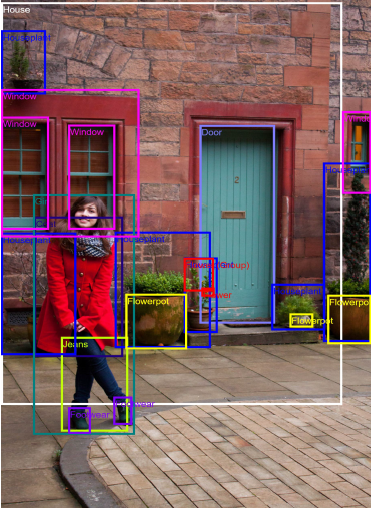
\includegraphics[width=0.7\textwidth]{images/image_example.PNG}
				\caption{Regions and classes.
					\hbox{\scriptsize Credit:\thinspace{\small\itshape \cite{liu_deep_2019}}}}
			\end{figure}
		\end{column}
	\end{columns}
\end{frame}


\subsection{RCNN: Girshick \it{et al. \cite{girshick_rich_2014}}}
\begin{frame}{}
	\begin{columns}
	% Column 1
		\begin{column}{0.5\textwidth}
			In 2013, Girshick proposed CNN for object detection.
			\begin{enumerate}
				\item[1] \emph{Region proposal computation}: Class agnostic region proposals via selective search.
				\item[2] \emph{CNN model finetuning}: Finetuning CNN pretrained model with region proposals, cropped from the image and warped into the same size.
			\end{enumerate}
		\end{column}
		% Column 2    
		\begin{column}{0.5\textwidth}
			\begin{figure}
				\centering
				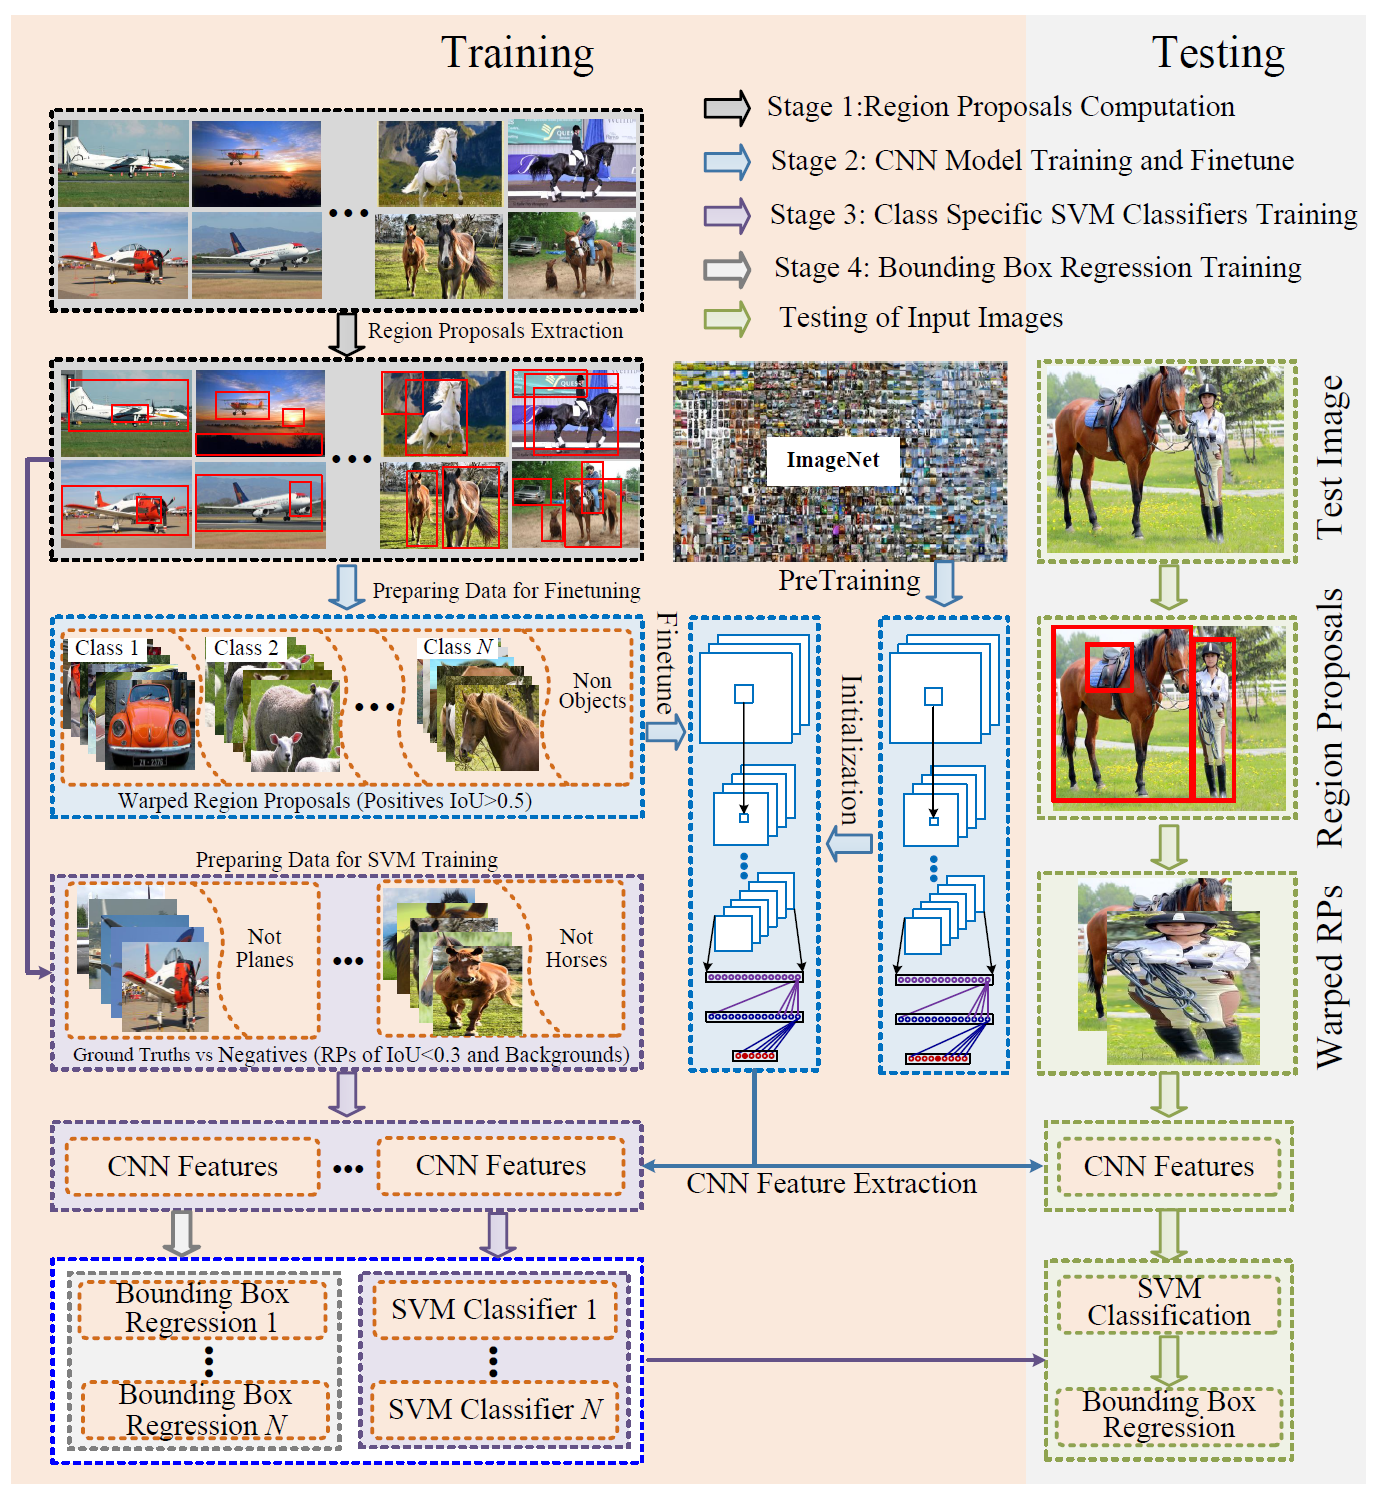
\includegraphics[width=0.9\textwidth]{images/RCNN.PNG}
				\caption{RCNN.
				\hbox{\scriptsize Credit:\thinspace{\small\itshape \cite{liu_deep_2019}}}}
			\end{figure}
		\end{column}
	\end{columns}
\end{frame}

\begin{frame}{}
	\begin{columns}
		% Column 1
		\begin{column}{0.5\textwidth}
			\begin{enumerate}
				\item[3] \emph{Class specific SVM classifiers training}. A set of class specific linear SVM classifiers are trained using fixed length features extracted with CNN, replacing the softmax classifier learned by finetuning.
				\item[4] \emph{Class specific bounding box regressors training}. Bounding box regression is learned for each object class with CNN features.
			\end{enumerate}
		\end{column}
		% Column 2    
		\begin{column}{0.5\textwidth}
			\begin{figure}
				\centering
				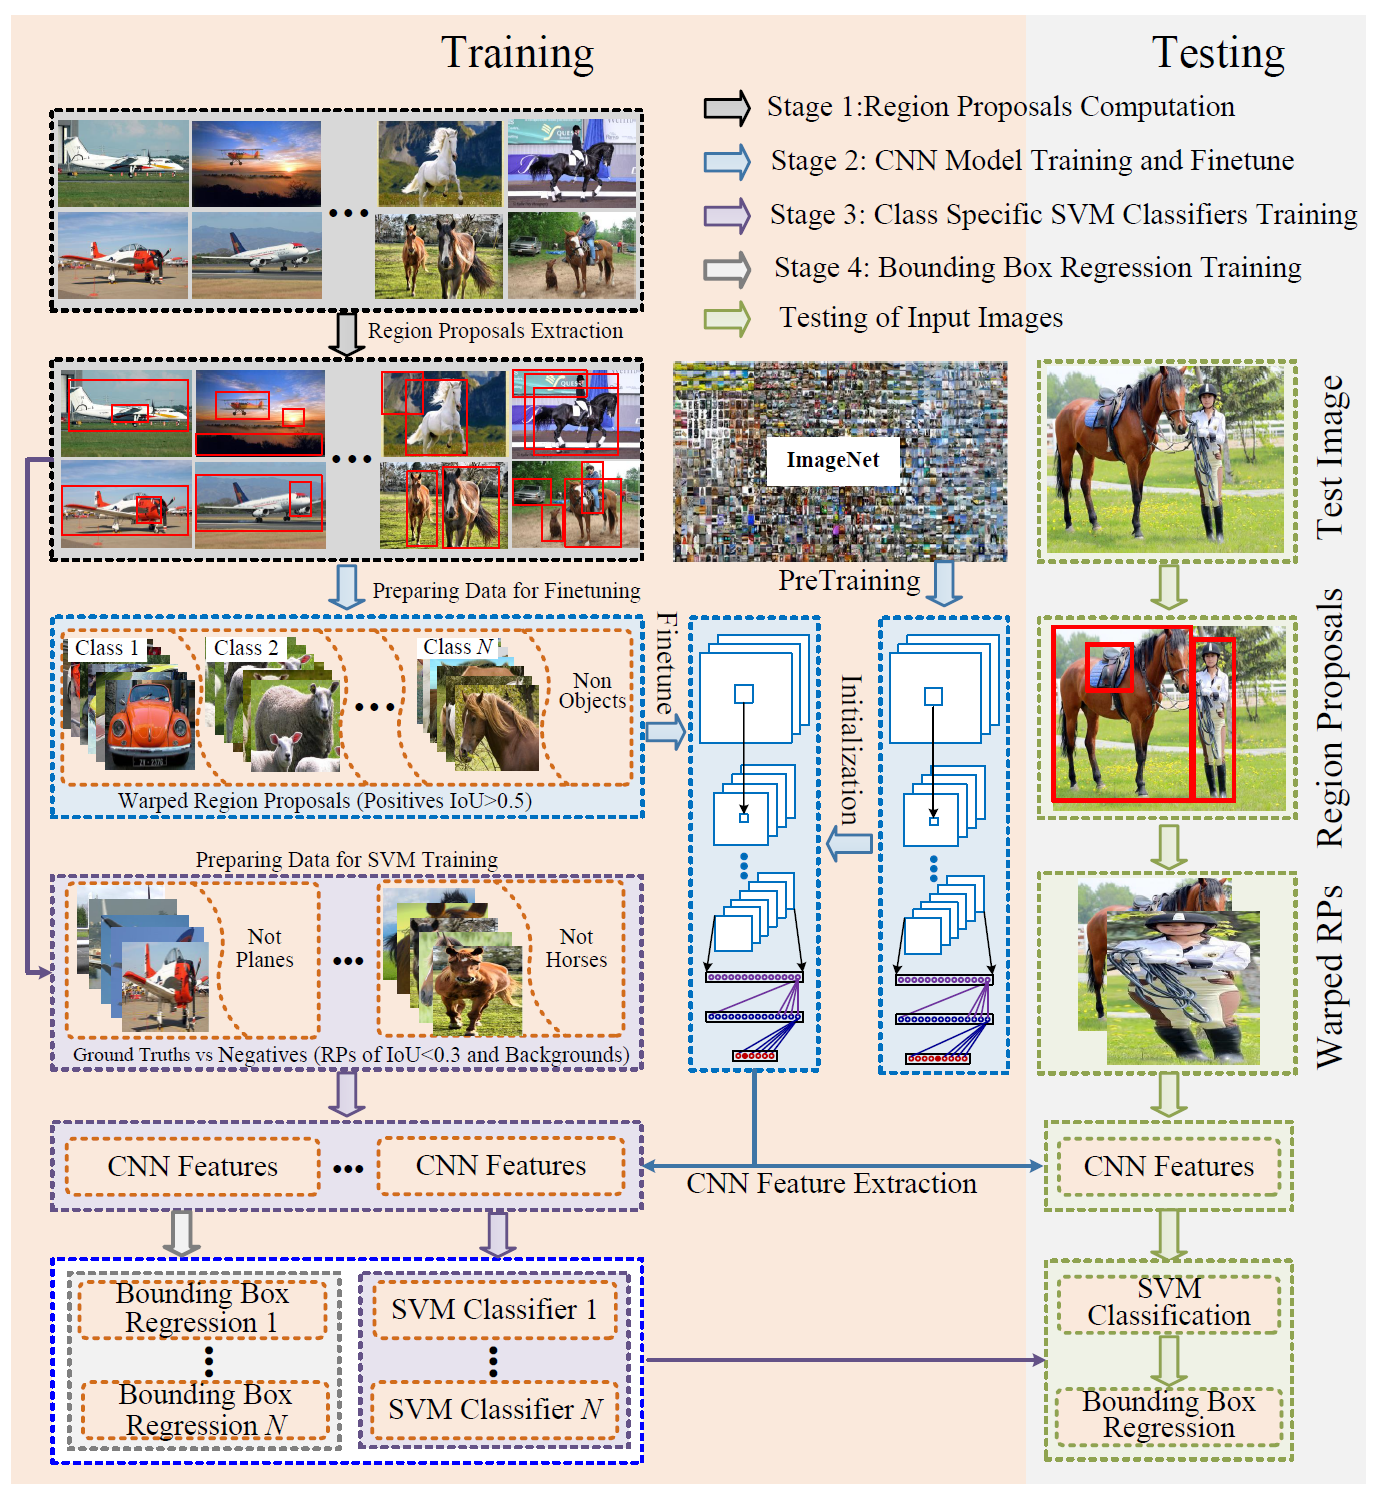
\includegraphics[width=0.9\textwidth]{images/RCNN.PNG}
				\caption{RCNN.
					\hbox{\scriptsize Credit:\thinspace{\small\itshape \cite{liu_deep_2019}}}}
			\end{figure}
		\end{column}
	\end{columns}
\end{frame}

\begin{frame}{Drawbacks}
	\begin{enumerate}
		\item Each individual stage must be trained separately which is slow and hard to optimize.
		\item For SVM classifier and bounding box regressor training, it is expensive in both disk space and time, because CNN features need to be extracted from each object proposal in each image and saved to disk, posing great challenges for large scale detection.
		\item Testing is slow, since CNN features are extracted per object proposal in each testing image, without sharing computation.
	\end{enumerate}
\end{frame}


\subsection{Fast RCNN: Girshick \cite{girshick_fast_2015}}
\begin{frame}{}
	\begin{columns}
		% Column 1
		\begin{column}{0.5\textwidth}
			\begin{itemize}
				\item Simultaneously learns a softmax classifier and a class-specific bounding box regression via 2 siblings output layers.
				\item Shares the computation of convolution across region proposals.
				\item Adds a Region of Interest (RoI) pooling layer between the last CONV layer and the first FC layer to extract a fixed-length feature for each region proposal. 
			\end{itemize}
		\end{column}
		% Column 2    
		\begin{column}{0.5\textwidth}
			\begin{figure}
				\centering
				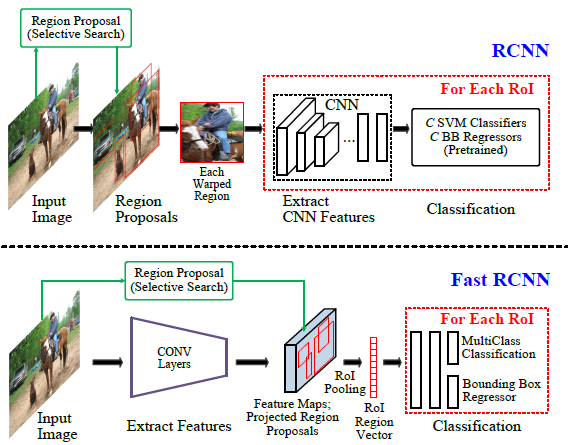
\includegraphics[width=0.9\textwidth]{images/rcnn-fastrcnn.PNG}
				\caption{From RCNN to Fast RCNN.
					\hbox{\scriptsize Credit:\thinspace{\small\itshape \cite{liu_deep_2019}}}}
			\end{figure}
		\end{column}
	\end{columns}
\end{frame}

\begin{frame}{}
	\begin{columns}
		% Column 1
		\begin{column}{0.5\textwidth}
			\begin{itemize}
				\item 3 times faster in training and 10 times faster in testing than RCNN.
				\item In summary:
				\begin{itemize}
					\item higher detection quality,
					\item single-stage training process that updates all network layers,
					\item no storage required for feature caching.
				\end{itemize}
			\end{itemize}
		\end{column}
		% Column 2    
		\begin{column}{0.5\textwidth}
			\begin{figure}
				\centering
				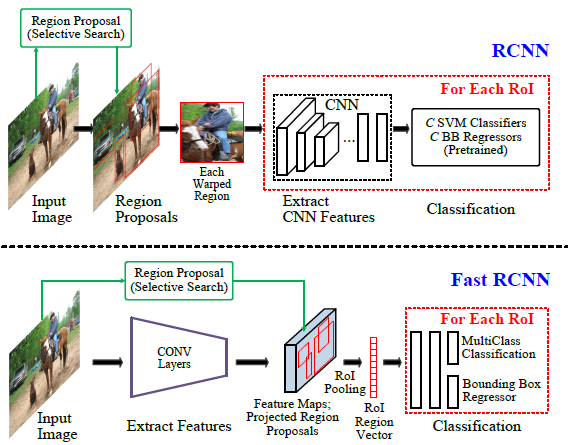
\includegraphics[width=0.9\textwidth]{images/rcnn-fastrcnn.PNG}
				\caption{From RCNN to Fast RCNN.
					\hbox{\scriptsize Credit:\thinspace{\small\itshape \cite{liu_deep_2019}}}}
			\end{figure}
		\end{column}
	\end{columns}
\end{frame}


\subsection{A word on RoI Pooling}
\begin{frame}{}
	Region of interest pooling is used to generate fixed-sized feature maps from CONV features maps to be used in FC layers. For example we want to RoI pool from a single 8×8 feature map, one region of interest (big black square) to an output feature map of 2×2.
	\begin{columns}
		% Column 1
		\begin{column}{0.7\textwidth}
			\begin{figure}
				\centering
				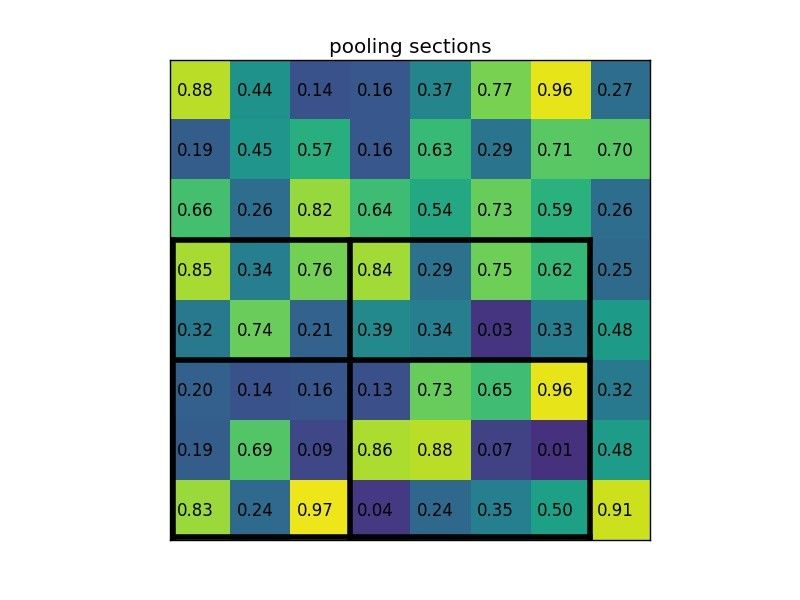
\includegraphics[width=0.9\textwidth]{images/pooling_sections.png}
			\end{figure}
		\end{column}
		\begin{column}{0.3\textwidth}
			\begin{figure}
				\centering
				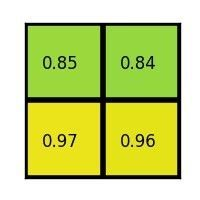
\includegraphics[width=0.9\textwidth]{images/roi_pooling.png}
			\end{figure}
		\end{column}
	\end{columns}
\end{frame}


\subsection{Faster RCNN: Ren \it{et al.} \cite{ren_faster_2015}}
\begin{frame}{}
	\begin{columns}
		% Column 1
		\begin{column}{0.5\textwidth}
			\begin{itemize}
				\item Selective Search (speed bottleneck) replaced by a CNN in producing region proposals, efficient and accurate Region Proposal Network (RPN).
				\item Same backbone network to accomplish the task of RPN for region proposal and Fast RCNN for region classification.
			\end{itemize}
		\end{column}
		% Column 2    
		\begin{column}{0.5\textwidth}
			\begin{figure}
				\centering
				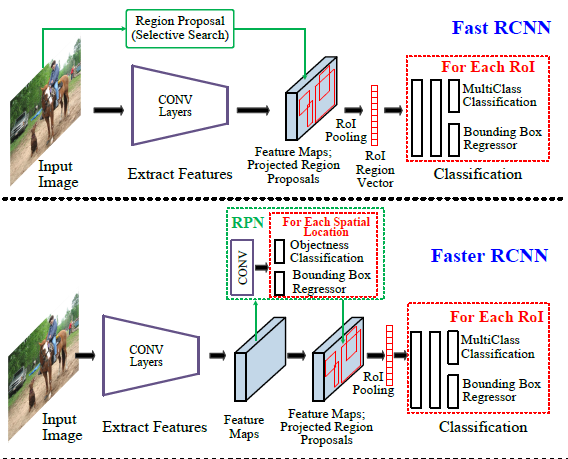
\includegraphics[width=0.9\textwidth]{images/fastrcnn-fasterrcnn.PNG}
				\caption{From Fast RCNN to Faster RCNN.
					\hbox{\scriptsize Credit:\thinspace{\small\itshape \cite{liu_deep_2019}}}}
			\end{figure}
		\end{column}
	\end{columns}
\end{frame}


\subsection{A word on RPN}
\begin{frame}{}
	We use RPN for:
		\begin{itemize}
			\item \emph{image classification}: generate the candidate boxes (which might have our objects to detect) and classify those boxes as one of the objects.
			\item \emph{bounding box regression}: box shape adjustments learn to properly fit the actual object.
		\end{itemize}
	This is done in three steps:
		\begin{enumerate}
			\item Generate anchor boxes.
			\item Classify each anchor box whether it is foreground or background.
			\item Learn the shape offsets for anchor boxes to fit them for objects.
		\end{enumerate}
\end{frame}

\begin{frame}{Anchor boxes}
	\begin{itemize}
		\item Every point in the feature map generated by the backbone network is an anchor point.
		\item From these points we generate candidate boxes using two parameters — scales and aspect ratios.
		\item The boxes need to be at image dimensions, whereas the feature map is reduced depending on the backbone.
		\item Ex: If anchor scales are [8,16,32] and ratios are [0.5,1,2] and stride is 16, then we use the combination of these scales and ratios to generate 9 anchor boxes for each anchor point and then take a stride of 16 over the image to take the next anchor box.
	\end{itemize}
\end{frame}

\begin{frame}{Anchor boxes}
	\begin{columns}
		% Column 1
		\begin{column}{0.5\textwidth}
			\begin{figure}
				\centering
				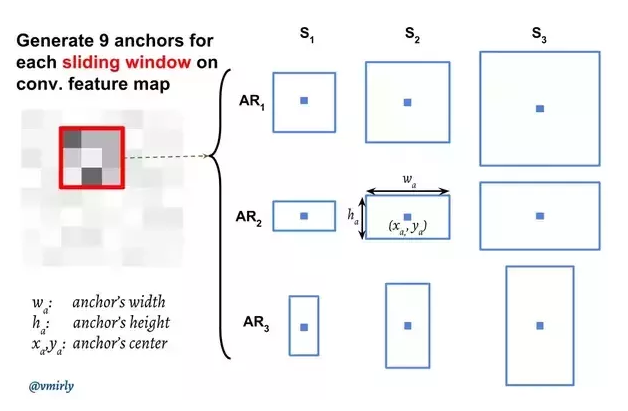
\includegraphics[width=0.9\textwidth]{images/anchor_boxes.png}
				\caption{Anchor boxes generation.}
			\end{figure}
		\end{column}
		\begin{column}{0.5\textwidth}
			\begin{figure}
			\centering
			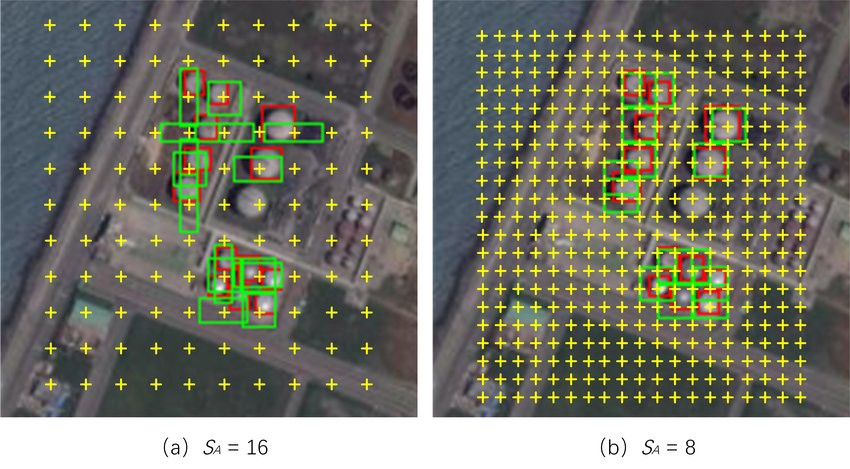
\includegraphics[width=0.9\textwidth]{images/anchor_boxes_images.jpeg}
			\caption{Anchor points with different scales.}
		\end{figure}
		\end{column}
	\end{columns}
\end{frame}

\begin{frame}{Foreground/Background and Bbox regression}
	\begin{columns}
		% Column 1
		\begin{column}{0.45\textwidth}
			\begin{itemize}
				\item Learn whether the given box is foregroud (object) or background and the offsets for the foreground boxes to adjust for fitting the objects.
				\item These tasks are achieved by two convolution layers on the feature map obtained from the backbone network.
			\end{itemize}
		\end{column}
		% Column 2    
		\begin{column}{0.55\textwidth}
			\begin{figure}
				\centering
				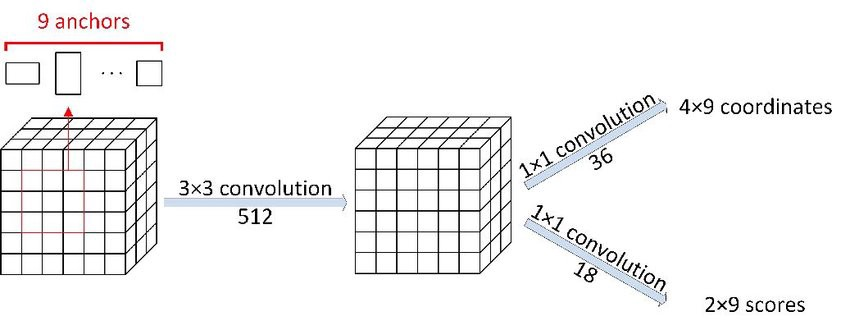
\includegraphics[width=0.9\textwidth]{images/rpn_networks.jpeg}
				\caption{2 scores (fg and bg) and 4 offsets for coordinates.}
			\end{figure}
		\end{column}
	\end{columns}
\end{frame}

\begin{frame}{Foreground/Background and Bbox regression}
	\begin{itemize}
		\item In anchor target generation, we calculate the IOU of GT boxes with anchor boxes to check if it is fg/bg and then the difference in the coordinates are calculated as targets to be learned by the regressor. Then these targets are used as input for cross-entropy loss and smooth l1 loss.
		\item Once these fg/bg scores and offsets are learned using convolution layers, some portions of fg and bg boxes are considered according to confidence scores. The offsets are applied to those boxes to get the actual ROIs to be processed further. This post-processing of anchor boxes using offsets is called proposal generation.
	\end{itemize}
\end{frame}


\section{Unified (One Stage) Frameworks}


\subsection{Philosophy}
\begin{frame}{}
	\begin{itemize}
		\item Region-based approaches are computationally expensive for current mobile/wearable devices.
		\item Instead of trying to optimize individual components of a complex region-based frameworks, researchers have begun to develop \emph{unified} detection strategies.
		\item Directly predict classes probabilities and bouding box offsets from full images with a single feed-forward CNN in a monolithic setting that does net involve region proposal generation of post classification / feature resampling, encapsulating all computation in a single network.
	\end{itemize}
\end{frame}


\subsection{Overfeat: Sermanet \it{et al.} \cite{sermanet_overfeat_2013}}
\begin{frame}{}
	\begin{itemize}
		\item First single-stage object detectors based on fully convolutional deep networks.
		\item Performs object detection via a single forward pass though the fully convolutional layers in the network.
		\begin{enumerate}
			\item Generate object candidates by performing object classification via a sliding window fashion on multiscale images.
			\item Increase the number of predictions by offset max pooling.
			\item Bounding box regression.
			\item Combine predictions using greedy merge strategy.
		\end{enumerate}
		\item Overfeat has a significant speed advantage, but is less accurate than RCNN.
		\item Difficult to train fully convolutional networks at the time.
	\end{itemize}
\end{frame}

\begin{frame}{}
	\begin{figure}
		\centering
		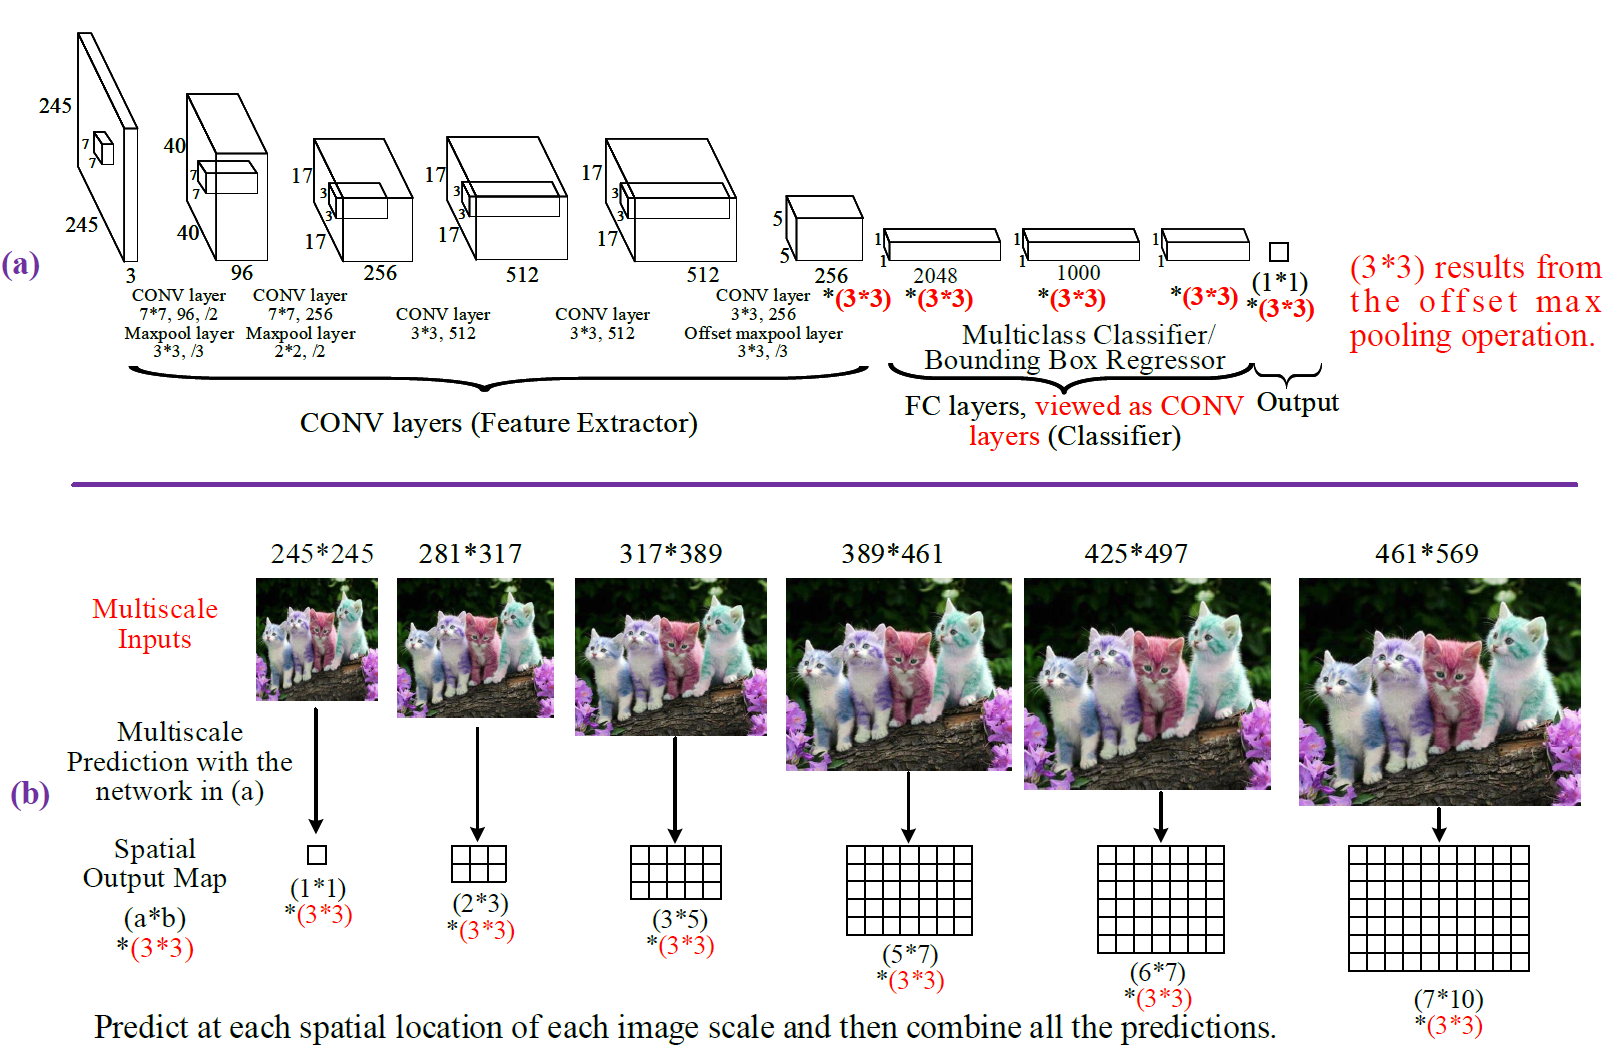
\includegraphics[width=0.9\textwidth]{images/overfeat.png}
		\caption{Overfeat.
			\hbox{\scriptsize Credit:\thinspace{\small\itshape \cite{liu_deep_2019}}}}
	\end{figure}
\end{frame}


\subsection{YOLO - You Only Look Once: Redmon \it{et al.} \cite{redmon_you_2016}}
\begin{frame}{}
	\begin{itemize}
		\item Directly predicts detections using a small set of candidate regions.
		\item Divides an image into an $S x S$ grid, each predicting $C$ class probabilities, $B$ bounding box locations, and confidence scores.
		\item Uses GoogLeNet as backbone.
		\item Sees the entire image, encodes contextual information about object classes, is less likely to predict false positives in the backgroud.
	\end{itemize}
	\begin{figure}
		\centering
		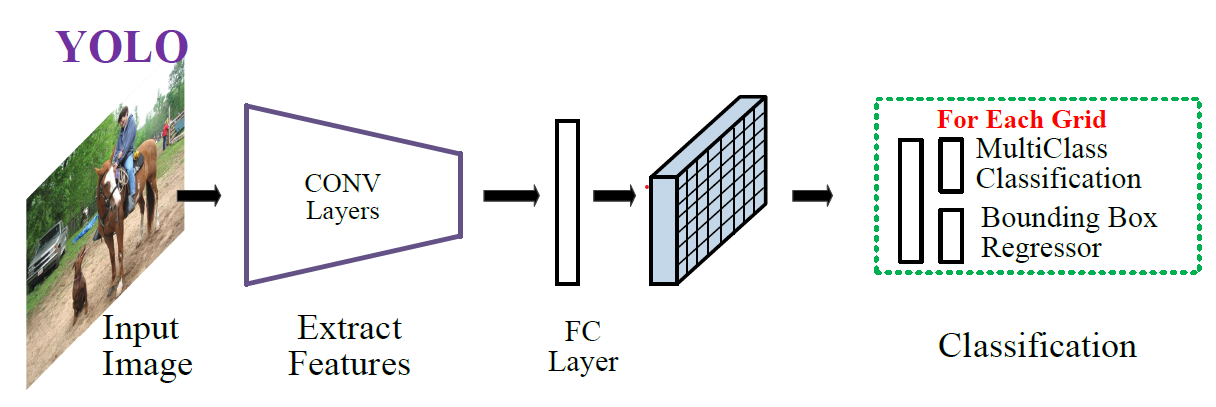
\includegraphics[width=0.7\textwidth]{images/yolo.png}
		\caption{YOLO.
			\hbox{\scriptsize Credit:\thinspace{\small\itshape \cite{liu_deep_2019}}}}
	\end{figure}
\end{frame}


\subsection{YOLOV2 and YOLO9000: Redmon and Farhadi \cite{redmon_yolo9000_2016}}
\begin{frame}{}
	YOLOV2 Improves YOLO:
	\begin{itemize}
		\item Custom GoogLeNet is replaced with the simpler DarkNet19 plus batch normalization.
		\item Anchor boxes are learned via kmeans and multiscale training.
	\end{itemize}
	YOLO9000 can detect over 9000 object categories in real time
	\begin{itemize}
		\item Joint optimization method to train simultaneously on an ImageNet classification dataset and a COCO detection dataset.
		\item Allow to perform weakly supervised detection (detecting object classes that do not have bounding boxes annotations)
	\end{itemize}
\end{frame}


\subsection{SSD - Single Shot Multibox Detector: Liu \it{et al.} \cite{liu_ssd_2016}}
\begin{frame}{}
	Combines ideas from RPN (competitive accuracy), YOLO (but faster) and multiscale CONV features.
	\begin{itemize}
		\item CNN fully convolutional, early stages based on a standard architecture such as VGG.
		\item Several auxiliary CONV layers, progressively decreasing in size.
		\item Information on the last layer may be too coarse spatially to allow precise localization so SSD performs detection over multiple scales.
		\item Uses Non-Maximum Suppression (NMS) step to produce final detection.
	\end{itemize}
	\begin{figure}
		\centering
		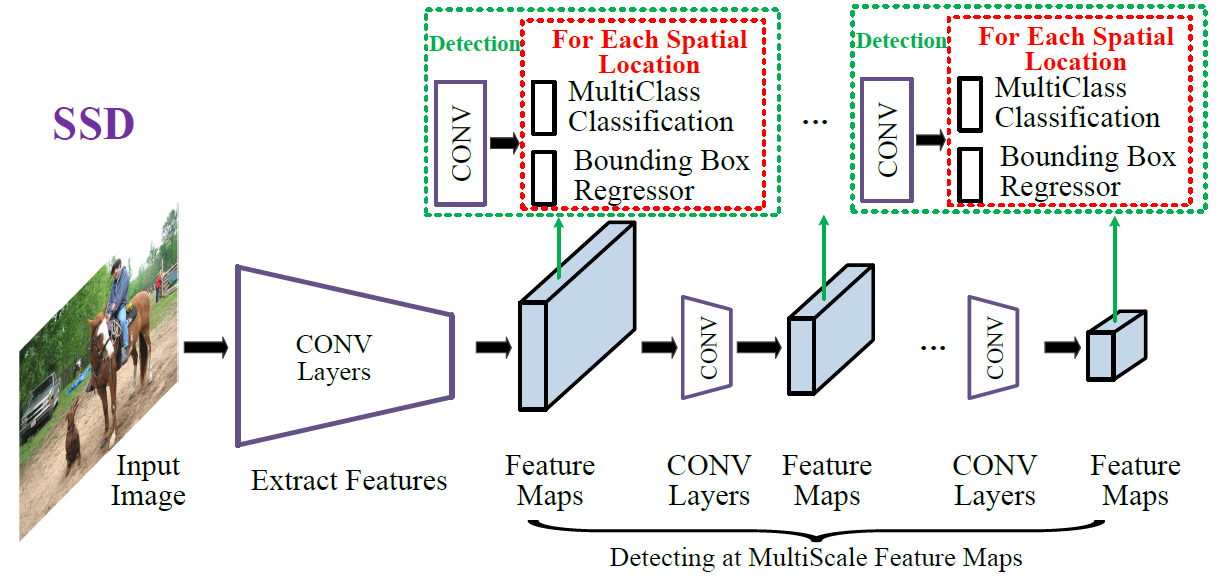
\includegraphics[width=0.55\textwidth]{images/ssd.png}
		\caption{SSD.
			\hbox{\scriptsize Credit:\thinspace{\small\itshape \cite{liu_deep_2019}}}}
	\end{figure}
\end{frame}

\begin{frame}{A word on Non-Maximum Suppression}
	\begin{columns}
		% Column 1
		\begin{column}{0.6\textwidth}
			\begin{figure}
				\centering
				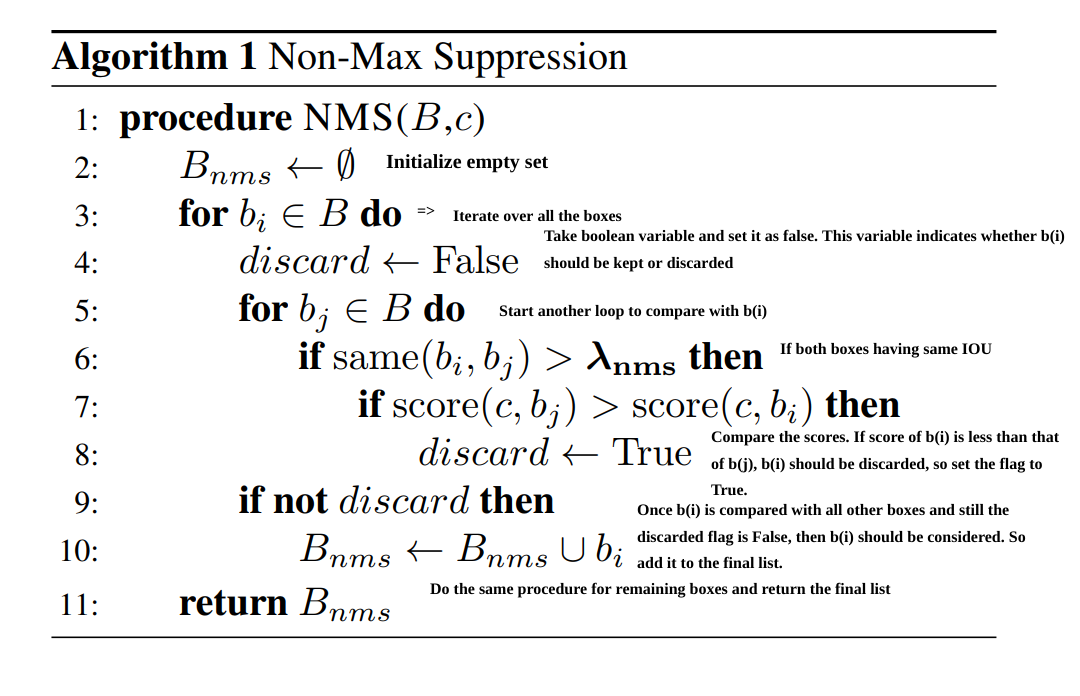
\includegraphics[width=\textwidth]{images/nms_algo.png}
				\caption{Algorithm}
			\end{figure}
		\end{column}
		\begin{column}{0.4\textwidth}
			\begin{figure}
				\centering
				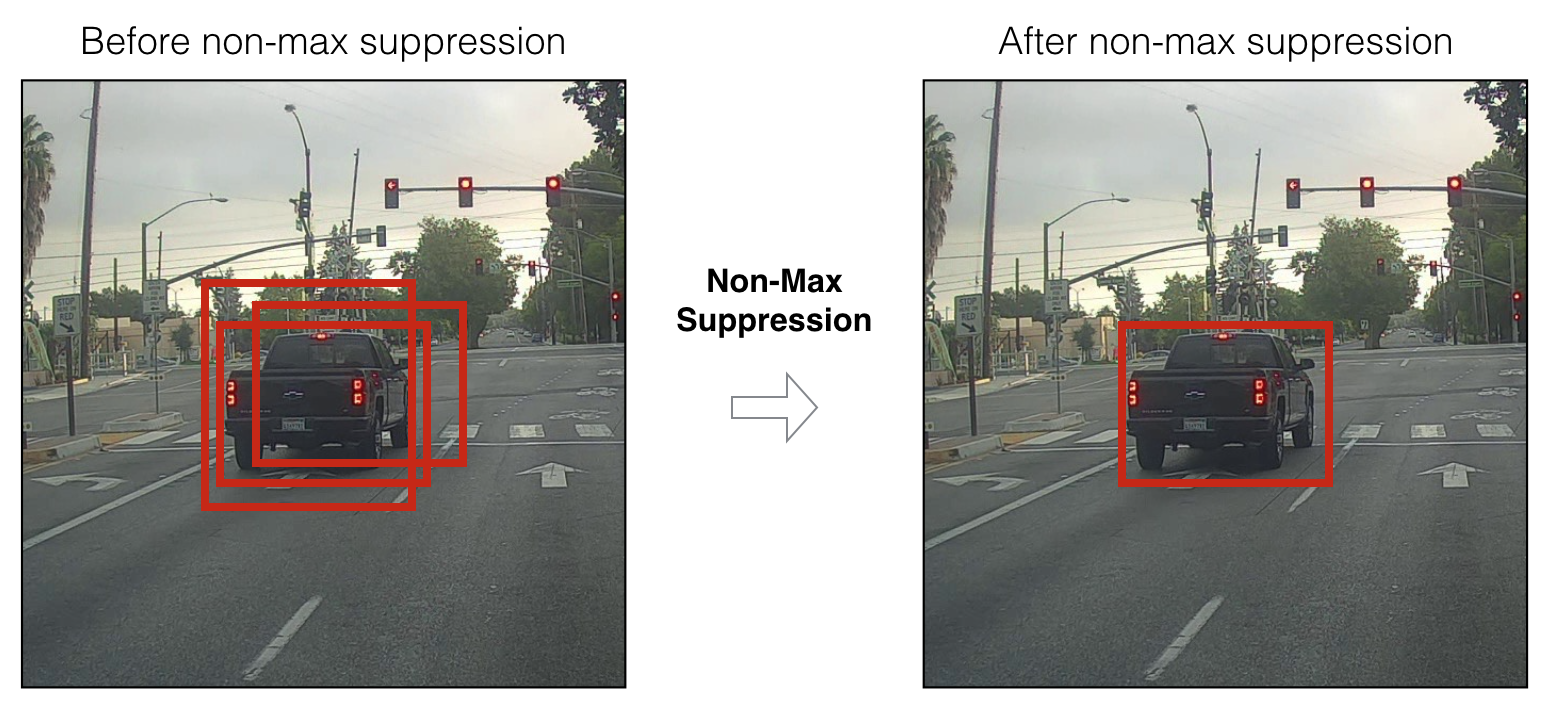
\includegraphics[width=\textwidth]{images/nms.png}
				\caption{result}
			\end{figure}
		\end{column}
	\end{columns}
\end{frame}

\part{Industry advices}
\begin{frame}
	\partpage
\end{frame}

\begin{frame}{Questions to answer before working}
	\begin{itemize}
		\item What is the target ? What should you detect ?
		\item What is the hardware to run the detector on ?
		\item Is there any annotated data ? Is there a way to get some ? Is there any open dataset on the subject ?
		\item Do I work from scratch or reuse the work of a colleague/GitHub ?
		\item Is there a minimal performance/accuracy to achieve ? A test/scenario the detector must pass ?
	\end{itemize}
\end{frame}

\begin{frame}{Advices}
	\begin{itemize}
		\item Annotate data is very long. It should be avoided as soon as is it possible.
		\item But bad labels will end in bad models. Be sure of the quality or your data.
		\item Iterate/version your model.
	\end{itemize}
	\begin{figure}
		\centering
		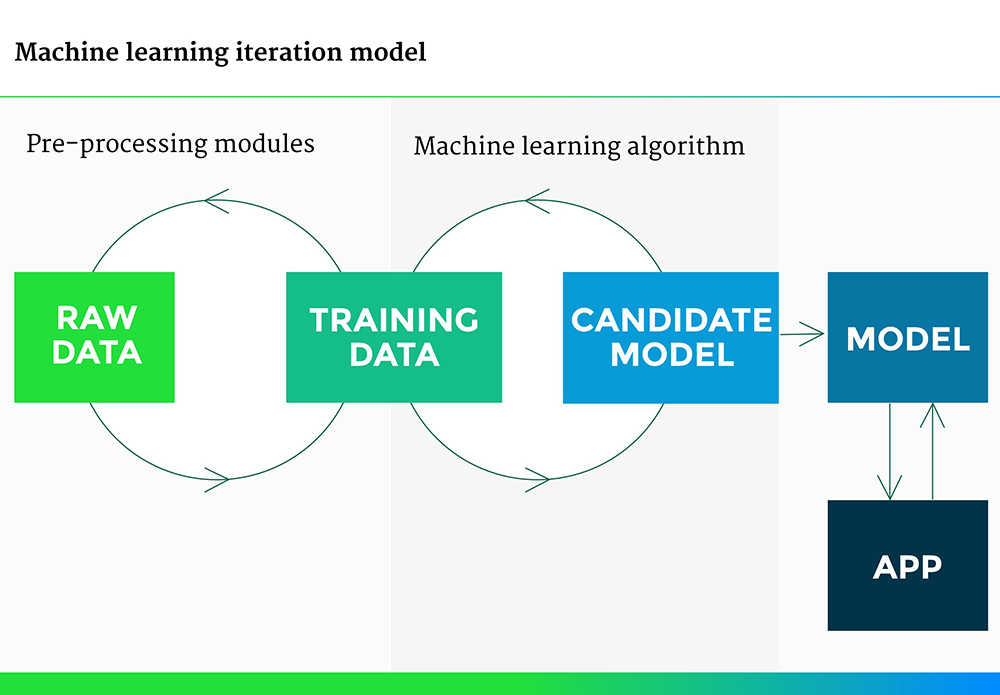
\includegraphics[width=0.6\textwidth]{images/iteration.jpg}
		\caption{Iterative process}
	\end{figure}
\end{frame}

\begin{frame}{Advices}
	\begin{columns}
		% Column 1
		\begin{column}{0.6\textwidth}
			\begin{itemize}
				\item Communicate your work. Use jupyter notebooks, dashboards, graphs, ...
				\item Evaluation metrics are very useful to monitor your model and the training process but not for communicating with non specialists.
				\item A demonstration is better than tables of numbers.
				\item Use docker to ease the deployment of your environment and allow IT teams to put your model into production.
			\end{itemize}
		\end{column}
		\begin{column}{0.4\textwidth}
			\begin{figure}
				\centering
				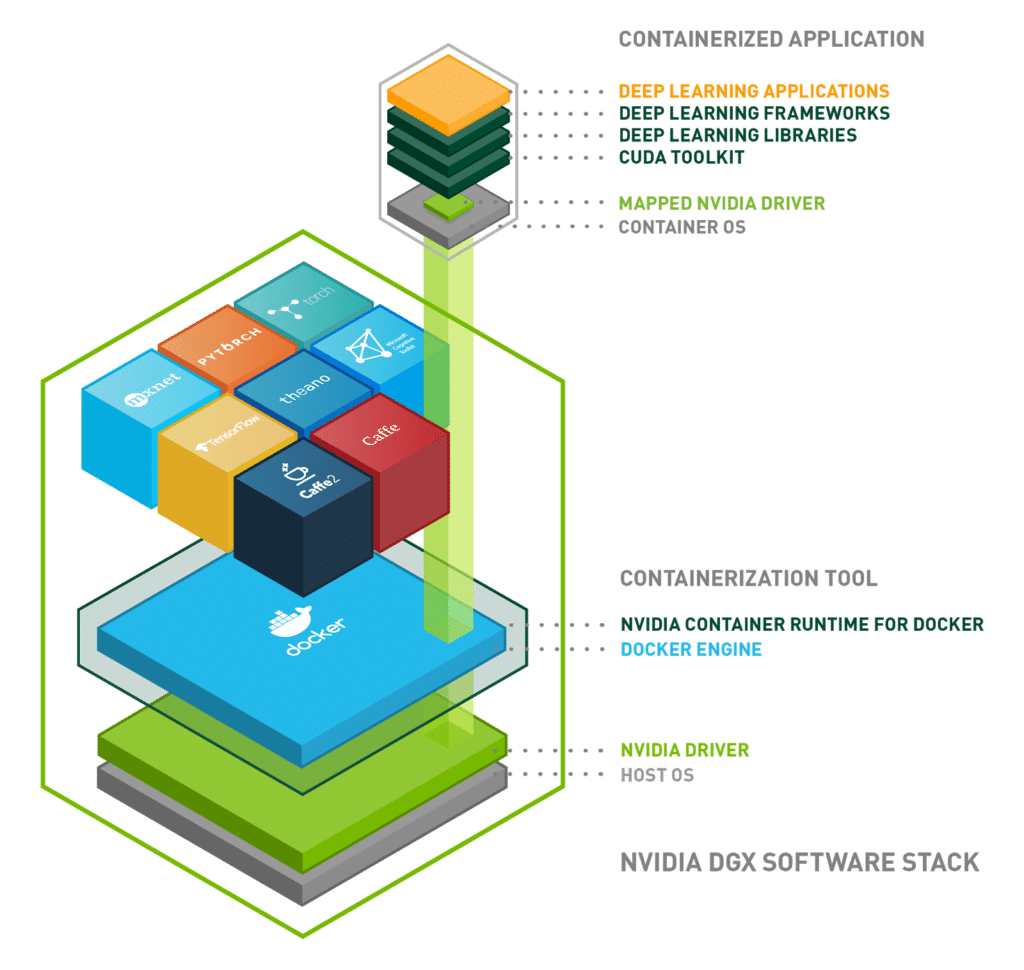
\includegraphics[width=0.9\textwidth]{images/docker.png}
				\caption{Docker
				\hbox{\scriptsize Credit:\thinspace{\small\itshape Nvidia}}}
			\end{figure}
		\end{column}
	\end{columns}
\end{frame}


\part{TP}
\begin{frame}
	\partpage
\end{frame}


\begin{frame}{}
	\begin{itemize}
		\item Link to google colab
	\end{itemize}
\end{frame}

\begin{frame}[allowframebreaks]
    \printbibliography
\end{frame}

\end{document}
